\chapter{Analysis of Timpani Percussion Performances}
\markboth{Analysis of Timpani Percussion Performance}{Analysis of Timpani Percussion Performance}
\label{chapter:Analysis}


%%%%%%%%%%%%%%%%%%%%%%%%%%%%%%%%%%%%%%%%%%%%%%%%%%%%%%%%%%%%%%%%%%%%%%%%%%%%%%%%%%%%%%%%%%%%%%%%%%%%%%%%%%%%%%%%%%%%

%In recent years, the control of virtual instruments or sound-synthesis processes by natural gestures has become an important research field, both for building new audio-visual tools and for exploring gesture-sound relationships. The goals of such multimodal and interactive tools are typically twofold, on the one hand it provides realistic virtual instruments whose response can be compared to real musical instruments, and on the other hand it gives the possibility to vary some input characteristics of natural gestures, while ensuring a certain coherence between gesture output and sound input parameters.\\

In this chapter, we present the explicit extraction of characteristics of natural percussion gestures. The analysis of pre-recorded percussion (timpani) gestures leads to the identification of significant parameters characterizing percussion playing techniques. The presented parameterization is also evaluated, showing that such parameters are consistent for discriminating the percussion playing techniques under study.\\

The chapter is organized as follows. We initially introduce a general description of timpani playing techniques in section \ref{sec:Analysis_TimpaniBasics}, as well as the building and pre-processing of a motion capture database of timpani percussion gestures in section \ref{sec:Analysis_MoCapDatabase}. We then present the extraction of the parameters that are used for discriminating percussion playing techniques, and we evaluate such a parameterization in section \ref{sec:Analysis_TimpaniAnalysis}. Finally, section \ref{sec:Analysis_Conclusion} finally concludes this analysis work on percussion playing techniques.

%%%%%%%%%%%%%%%%%%%%%%%%%%%%%%%%%%%%%%%%%%%%%%%%%%%%%%%%%%%%%%%%%%%%%%%%%%%%%%%%%%%%%%%%%%%%%%%%%%%%%%%%%%%%%%%%%%%%


%%%%%%%%%%%%%%%%%%%%%%%%%%%%%%%%%%%%%%%%%%%%%%%%%%%%%%%%%%%%%%%%%%%%%%%%%%%%%%%%%%%%%%%%%%%%%%%%%%%%%%%%%%%%%%%%%%%%

%	\section{Introduction and Motivation}
%	\label{sec:Analysis_Introduction}

%In playing a music instrument, the musician establishes a more or less continuous interaction with the instrument. This interaction is based on complex mechanims, allowing the fine-tuning of the sound-producing gestures via sensorimotor loops, including audio, visual and gestural feedbacks. Moreover, these sensory informations are directly influenced by the semantic information contained in the musical phrases, and may change the motor commands that produce the gesture. Virtual musical instruments controlled by natural gestures try to realistically reproduce this sensorimotor situation with the aims of, first approaching real instrumental situations, and second exploring the gesture-sound relationship. This reality may then be extended through new paradigms where users can interact in real-time with sound processes.\\

%Traditional acoustic models provide a formal representation of the underlying physical mechanisms that are at the origin of the produced sounds. Such models have been proposed for a wide range of musical instruments \citeCM{smith:JNMR05}, such as plucked \citeCM{laurson:CMJ01} or striked \citeCM{bensa:JAS03} strings, as well as single-reed \citeCM{kergomard95} or brasses instruments \citeCM{msallam:AAA00}. These contributions imply more generally inversion processes (\myfigname \ref{fig:VMIs-VG}), starting from the produced sound to physical parameters (inversion $I_1$) for controlling virtual instruments models, which are themselves driven by instrumental gesture excitations (inversion $I_2$, interaction gesture).\\

%Beyond the nature and the quality of previously cited models, one of the main issue of the above approaches is to characterize the inversion processes, and especially to map the physical parameters of the virtual instrument with interaction gestures. In a more extended approach, this question is adressed in terms of how sensory informations can be captured from natural gestures and what kind of mapping layers can be elaborated for taking these informations into account \citeCM{miranda:AR06}. This has led to the design of many new digital music instruments for exploring this problem, involving various types of sensor technologies applied to different musical tasks, such as percussion \citeCM{kapur:JNMR03}, violin \citeCM{demoucron:PhD08} or guitar \citeCM{pakarinen:CMJ08} performances. More recently, the growing interest to the analysis of musical performances \citeIPA{dahl:PhD05, rasamimanana:PhD08} attests the need of some \emph{a priori} knowledge about musical tasks, so that this mapping issue can find realistic and reliable solutions.\\

%\begin{figure}%[H]
%	\begin{center}
%	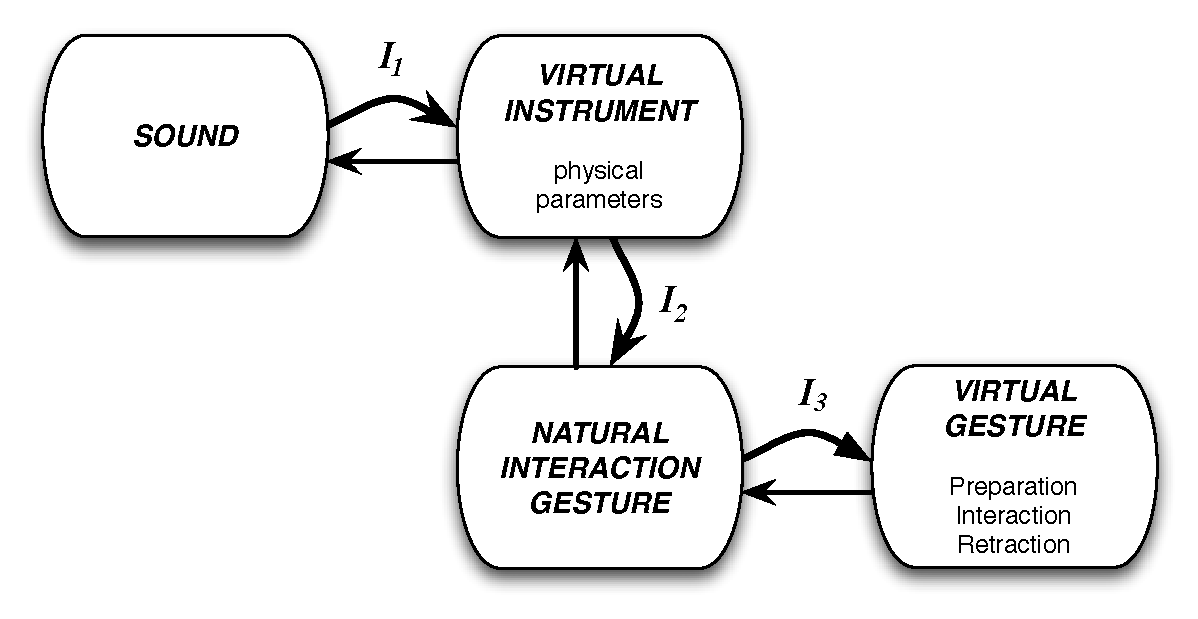
\includegraphics[width=0.6\textwidth]{Chapter4/Pics/Pdf/VirtualGesture.pdf}
%	\end{center}
%	\vspace{-1cm}
%	\caption{Inversion processes involved in the control of virtual instruments}
%	\label{fig:VMIs-VG}
%\end{figure}

%Our work takes place in the fact that there is a lack of knowledge on significant gestural characteristics that can be applied to virtual instruments producing sound. We therefore propose to go further and introduce a complete modeling of gesture, by designing a human-like character endowed with realistic and expressive behaviors. In order to reproduce the main characteristics of the control exerted on a real instrument, and more specifically the efforts involved in the interaction, we adopt a physics-based approach for modeling both the virtual performer and the sound-synthesis process (chapter \ref{chapter:Synthesis}). Such a physics modeling approach allows to represent not only what occurs during the mechanical interaction between the instrumentist and the instrument, but also the whole gesture production system, including the preparatory and the retraction phases that precede and follow the interaction process (\myfigname \ref{fig:VMIs-VG}, inversion $I_3$).

%Our work sensibly differs from the ones that use the gestural signals  directly responsible for the sound production \citeIPA{bevilacqua:NIME07}, as we build the physical model that produces these gestural signals. Such a modeling and simulation approach provides kinematics and dynamics information of the movement throughout the duration of the instrumental performance. It thus becomes possible to modify the biomechanical parameters of the virtual performer and change the simulated movement.\\

%However, without any real data, infering the forces and moments applied to joints and bones of the character still remains a difficult problem (inverse problem). We propose to solve it by using motion captured data recorded during real performances. The idea is to extract from these data a segmented and reduced-dimension representation of motion, and then to edit and assemble these motion chunks in order to control the virtual character. One key issue of our work is therefore to finely understand the underlying processes involved in the control of the virtual performer, and the way it is related to motion captured data recorded during real performances. In order to achieve these objectives, we highlight in an analysis process the significant dimensions of gesture that are involved when playing various percussion exercices. In particular we show that the mallet extremity trajectories may significantly characterize the gesture variations and may be used through an inversion process to control the virtual character.


%The main interest of a biomechanics-based modeling of gesture lies in the dynamical understanding of the mechanical links established between the instrumentist and the instrument. Furthermore, the physical approach may give some insight into the various parameters that are responsible for conducting specific performances with a desired expressivity. These parameters may characterize for example the joint constraints in the form of angular limits or biomechanical parameters such as stiffness, or damping of the joints. Finally, such a physics modeling approach allows to represent not only what occurs during the mechanical interaction between the instrumentist and the instrument, but also the whole gesture production system, including the preparatory and the retraction phases that precede and follow the interaction process (\myfigname \ref{fig:VMIs-VG}, inversion $I_3$).\\

%In the same way as the sound-synthesis research focuses on effect-centered (sampling and spectral modeling) or cause-centered (physical modeling) methods, the control of virtual characters involves either kinematics (effect-centered, see for instance \citeCGA{tolani:GM00}) or dynamics (cause-centered, for example \citeCGA{zordan:TOG05}) solutions. In order to take advantage of both methods, we define a cascaded combination of two inversion models (kinematics and dynamics) that allows to control the virtual performer through a sensorimotor control loop. This controller (\myfigname \ref{fig:gestureSoundProduction}) uses sensory informations (for example kinematic mallet trajectories or more generally visual information) to update the forces or torques that drive the muscular-skeleton model of the virtual performer. More related to musical gesture modeling, our work sensibly differs from the ones that use the gestural signals  directly responsible for the sound production \citeCM{bevilacqua:NIME07}, as we build the physical model that produces these gestural signals. Such a modeling and simulation approach provides kinematics and dynamics information of the movement throughout the duration of the instrumental performance. It thus becomes possible to modify the biomechanical parameters of the virtual performer and change the simulated movement.\\

%However, without any real data, infering the forces and moments applied to joints and bones of the character still remains a difficult problem (inverse problem). We propose to solve it by using motion captured data recorded during real performances. The idea is to extract from these data a segmented and reduced-dimension representation of motion, and then to edit and assemble these motion chunks in order to control the virtual character. One key issue of our work is therefore to finely understand the underlying processes involved in the control of the virtual performer, and the way it is related to motion captured data recorded during real performances. In order to achieve these objectives, we highlight in an analysis process the significant dimensions of gesture that are involved when playing various percussion exercices. In particular we show that the mallet extremity trajectories may significantly characterize the gesture variations and may be used through an inversion process to control the virtual character.

%\begin{figure}[H]
%	\begin{center}
%	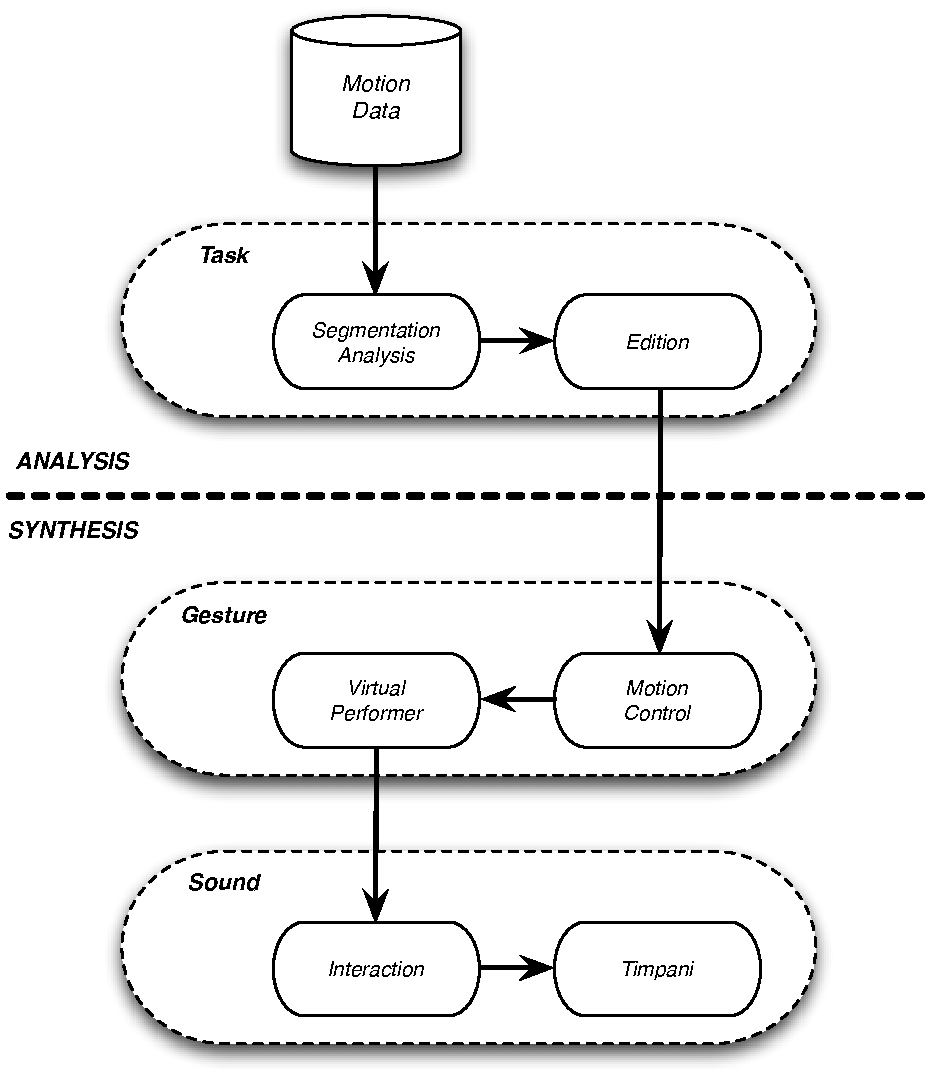
\includegraphics[width=0.6\textwidth]{./Data/Pdf/GeneralApproach-b&w.pdf}
%	\end{center}
%	\vspace{-1cm}
%	\caption{Gesture and sound production.}
%	\label{fig:gestureSoundProduction}
%\end{figure}

%The paper is organised as follows. Section \ref{sec:analysis} presents the extraction of a set of relevant parameters characterizing percussion performance, as well as its evaluation. We then propose a control method for synthesizing virtual percussion gestures in section \ref{sec:modelingControl}, based on the previous analysis stage. Results are then presented in section \ref{sec:results}; they concern both the evaluation of the synthesized gestures compared to real ones, and the visualization of the synthesized performances. We eventually conclude and draw perspectives of this work in section \ref{sec:conclusion}.

%%%%%%%%%%%%%%%%%%%%%%%%%%%%%%%%%%%%%%%%%%%%%%%%%%%%%%%%%%%%%%%%%%%%%%%%%%%%%%%%%%%%%%%%%%%%%%%%%%%%%%%%%%%%%%%%%%%%


%%%%%%%%%%%%%%%%%%%%%%%%%%%%%%%%%%%%%%%%%%%%%%%%%%%%%%%%%%%%%%%%%%%%%%%%%%%%%%%%%%%%%%%%%%%%%%%%%%%%%%%%%%%%%%%%%%%%

	\section{Timpani Basics}
	\label{sec:Analysis_TimpaniBasics}

There are many classifications of percussion instruments, one of the most established typologies is based on physical characteristics of instruments and the way by which they produce sound. According to this classification, timpani are considered as membranophones, "producing sound when the membrane or head is put into motion" \citeIPA{cook97}. Timpani are also called "kettledrums", and are considered as the first percussion instrument introduced in the composition of a classical orchestra more than 400 years ago \citeIPA{blades95}. The dramatic resounding and powerful effects that can emerge from the timpani makes this instrument one of most important percussion instrument in an orchestra.\\

In this subsection, we depict the basics for playing timpani, including the presentation of timpani-related equipments, acoustics properties of timpani sound properties, as well as its main playing techniques.


		\subsection{Equipment}
		\label{subsec:Analysis_TimpaniBasics_Equipment}

The equipment related to timpani is mainly composed of a bowl, a head and mallets as shown in \myfigname \ref{fig:timpaniEquipment}. In general, timpanists have to cope with several timpani (usually four) with bowls varying in size. The diameter of timpani membranes usually range from 23'' to 32'' \citeIPA{peters84} and players should properly tune each timpani to its corresponding pitch interval (\mytabname \ref{tab:timpaniPitch}).\\

As for timpani mallets, they consist of a shaft and a head. They are designed in various lengths, weights, thicknesses and materials \citeIPA{cook97} and their choice is of great importance \citeIPA{noak84}, namely depending on the percussionist level and on the task to be performed in the instrumental situation (low or fast rolls).

\begin{figure}%[H]
	\begin{center}
		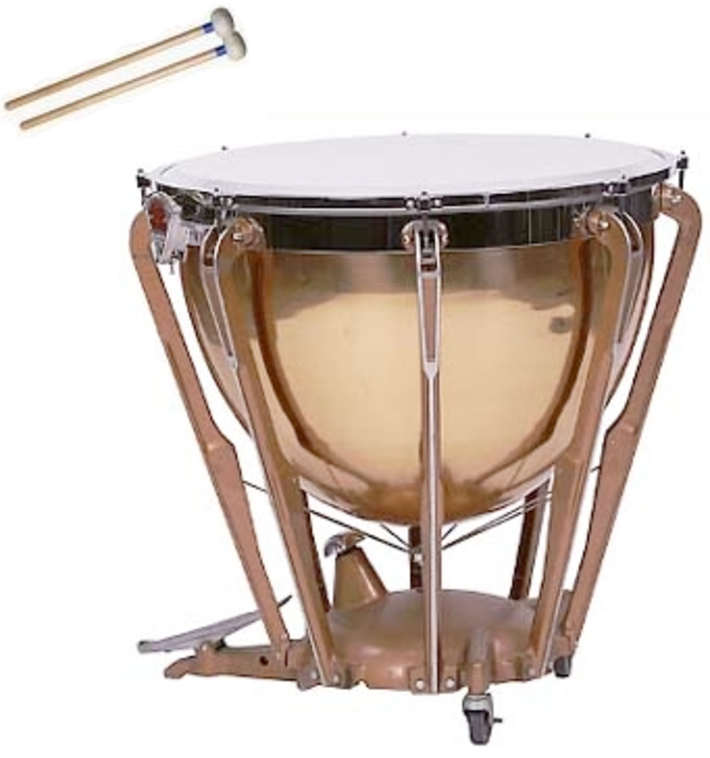
\includegraphics[width=0.4\columnwidth]{Chapters/4/Pics/Pdf/timpaniEquipment.pdf}
	\end{center}
	\vspace{-0.5cm}
	\caption[Timpani equipment]{Timpani equipment: bowl, membrane and mallets.}
	\label{fig:timpaniEquipment}
\end{figure}

\begin{table}%[H]
	\centering
	\caption[Bowl diameters and corresponding pitch intervals]{Bowl diameters and corresponding pitch intervals.}
	\vspace{2mm}
	\begin{tabular}{||x{3cm}||x{2cm}|x{2cm}|x{2cm}|x{2cm}||} \hline
		\small{$Bowl$ $diameter$} 	& $23''$ 	& $26''$ 	& $29''$ 	& $32''$	\tabularnewline \hline \hline
		\small{$Pitch$ $interval$} 	& $D3-A3$ 	& $B^b2-F3$ & $F2-C3$ 	& $D2-A2$	\tabularnewline \hline
	\end{tabular}
	\label{tab:timpaniPitch}
\end{table}


		\subsection{Acoustics}
		\label{subsec:Analysis_TimpaniBasics_Acoustics}

The acoustics of timpani percussion instruments has extensively been under study, mostly due to the timpani oddity known as the "missing fundamental" problem. The "missing fundamental" issue is well known among timpanists, this refers to the fact that a strike in the membrane center result in a muffled sound, so that the fundamental of timpani is considered to be the sound resulting from the '11' vibration mode rather than the '01' vibration mode (\myfigname \ref{fig:timpaniModes}). Other vibrating modes correspond to harmonics, such as the '21' and '31' modes which are respectively related to a fifth and a major seventh. It has been moreover shown that 'x1' vibration modes characterize predominant harmonic partials \citeIPA{rossing:SA82}. The "missing fundamental" issue can therefore be seen as a vibrating mode shift as the fundamental is shifted from the '01' mode to the '11'.\\

\begin{figure}[H]
	\begin{center}
		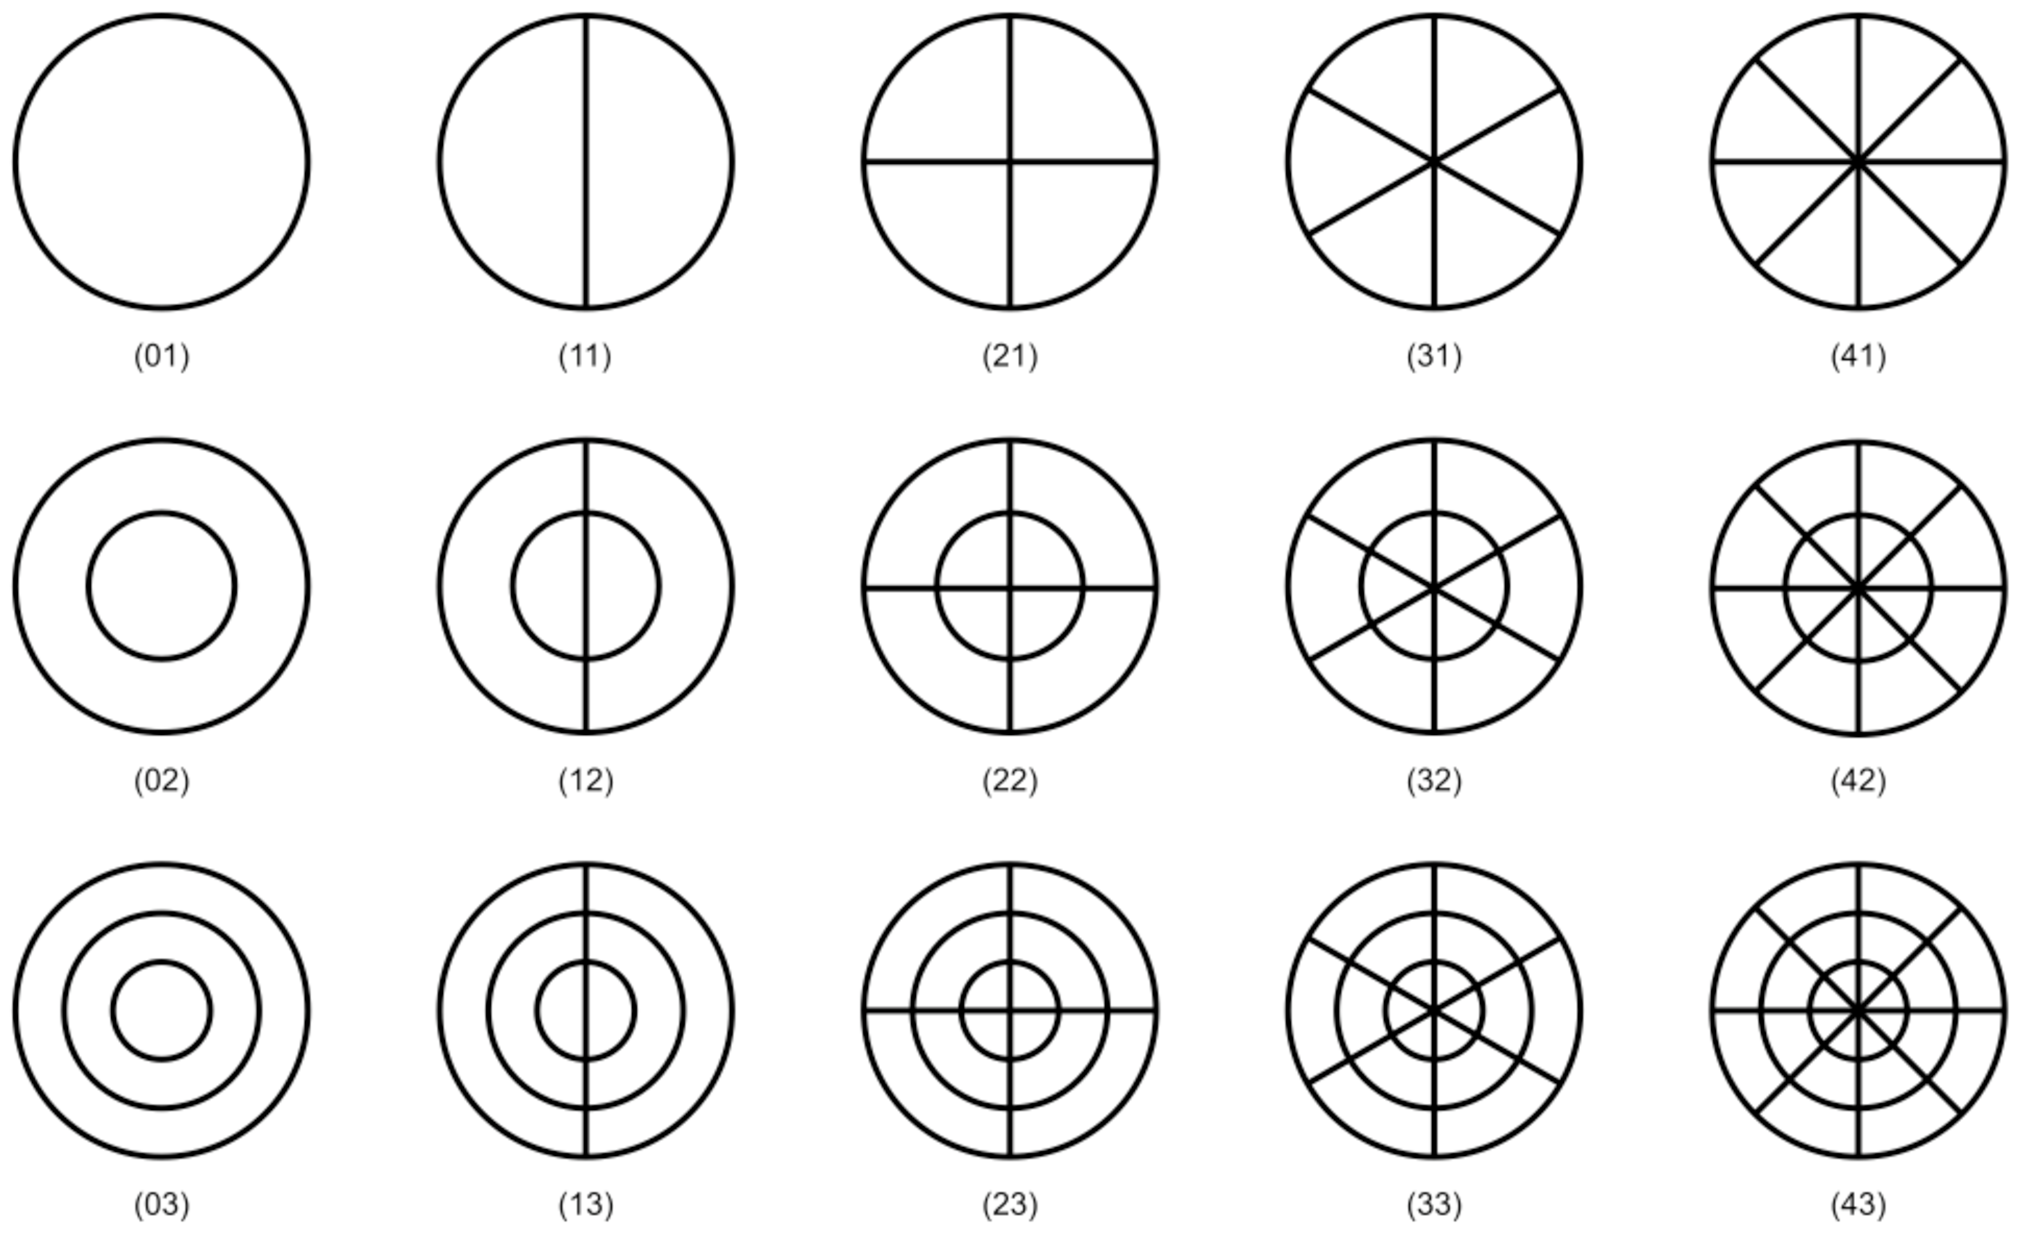
\includegraphics[width=0.8\columnwidth]{Chapters/4/Pics/Pdf/timpaniModes.pdf}
	\end{center}
	\vspace{-0.5cm}
	\caption[Vibrating modes of a timpani membrane]{Vibrating (x, y) modes of a timpani membrane, vertically (x) and horizontally (y)(courtesy of \citeIPA{rossing91}).}
	\label{fig:timpaniModes}
\end{figure}

\begin{figure}[H]
	\begin{center}
		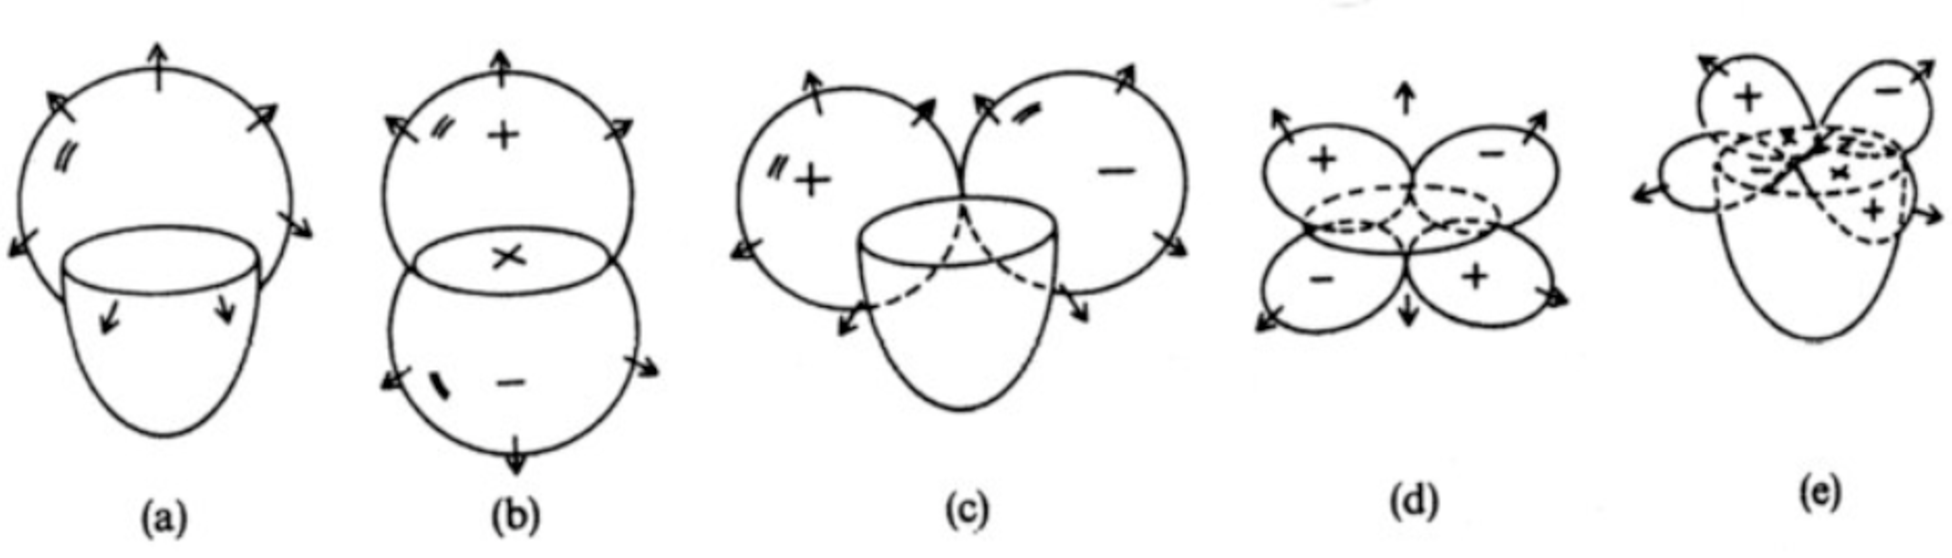
\includegraphics[width=0.8\columnwidth]{Chapters/4/Pics/Pdf/timpaniRadiationPoles.pdf}
	\end{center}
	\vspace{-0.5cm}
	\caption[Radiation poles of a timpani membrane]{Radiation poles of a timpani membrane: (a) monopole radiation of a baffled membrane in its (0, 1) mode, (b) dipole radiation of an unbaffled membrane in its (0, 1) mode, (c) dipole radiation of a baffled membrane in its (1, 1) mode, (d) quadrupole radiation of an unbaffled membrane in its (1, 1) mode, (d) quadrupole radiation of a baffled membrane in its (2, 1) mode (courtesy of \citeIPA{rossing91}).}
	\label{fig:timpaniRadiationPoles}
\end{figure}

The "missing fundamental" issue has also been explained in radiation terms. The most predominant phenomenon responsible of the vibrating mode shift is the air loading effect \citeIPA{rossing91} occuring in the timpani bowl. The radiated energy after a strike corresponding to the '01' is characterized by a monopole radiation scheme, so that the energy is radiated much more rapidly compared to other mode excitations (\myfigname \ref{fig:timpaniRadiationPoles}). Conversely other modes are radiating according to di- or quadrupoles that characterize lower radiation velocities.\\

The "missing fundamental" phenomenon is the reason why timpanists perform rarely a beat attack at the center of the timpani membrane. This observation is taken into account in our protocol for capturing timpani playing techniques, as we will see in the next section.

%\newpage


		\subsection{Playing Techniques}
		\label{subsec:Analysis_TimpaniBasics_Playing}

Timpani playing is characterized by a wide range of playing techniques, among them mallet grips as well as beat impact locations on the drum membrane are common features for differencing these techniques.\\

There are two main strategies for holding mallets, \myfigname \ref{fig:timpaniBasics1}: the \emph{French} grip (also called "thumbs-up") and the \emph{German} grip (or "matched" grip). These techniques imply different positions of the hand (vertical palm with the \emph{French} grip, horizontal with the \emph{German} grip), thus different motions of the wrist and of the fingers. 

Moreover, the use of the arms and forearms differ: broadly speaking, the \emph{French} grip asks for bigger amplitude in the use of the arms and forearms. It should be noted however that many timpanists use other techniques combining features from the two main techniques described here, or with a position of the wrist placing the palm at an angle of 45 degrees with the head of the timpani.\\

\begin{figure}%[H]
	\begin{center}
		\subfigure[]{\label{fig:timpaniBasics1}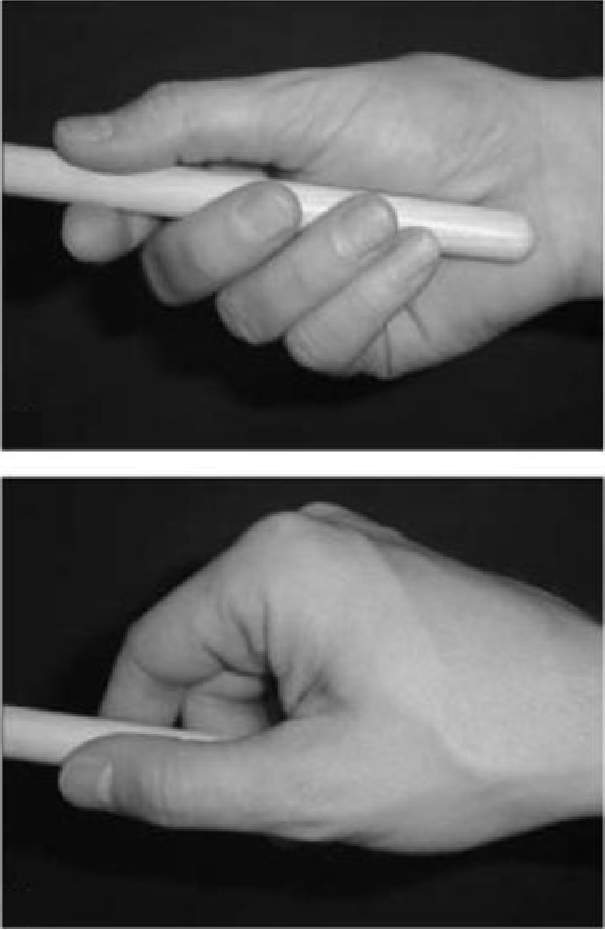
\includegraphics[width=0.25\columnwidth]{Chapters/4/Pics/Pdf/grips.pdf}}
		\subfigure[]{\label{fig:timpaniBasics2}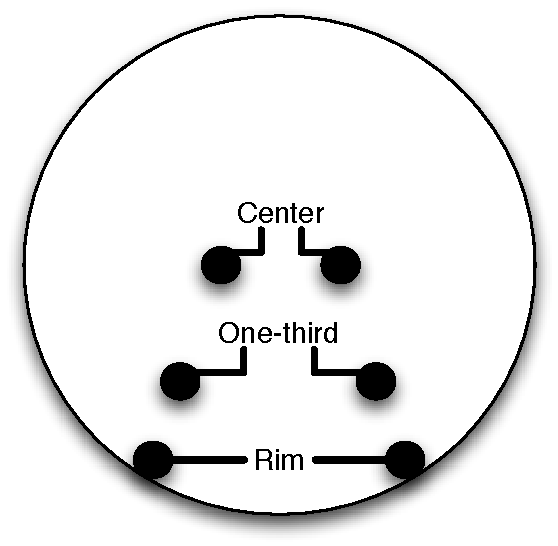
\includegraphics[width=0.35\columnwidth]{Chapters/4/Pics/Pdf/beatLocations2.pdf}}
	\end{center}
	\vspace{-0.5cm}
	\caption[Mallet grips and beat impact locations]{(a) \emph{French} (top) and \emph{German} (bottom) mallet grips. (b) Top view of the drum membrane: beat impact locations.}
	\label{fig:timpaniBasics}
\end{figure}

Moreover, players commonly use three distinct locations of impacts (\myfigname \ref{fig:timpaniBasics2}): \emph{One-third} of membrane radius, \emph{Center} and \emph{Rim} of the membrane. The most used is definitely the \emph{One-third} location, producing a full sound with a lot of resonance. The \emph{Center} location is characterized by a sharp and muffled attack with barely any resonance. And finally the \emph{Rim} location is characterized by a metallic sound and a resonance bringing mostly out high frequencies. These \emph{Center} and \emph{Rim} beat impact locations are used less often and have been adopted by composers after Eliot Carter's "Eight Pieces for Four Timpani" \citeIPA{carter68}.\\

\begin{figure}%[H]
	\begin{center}
		\subfigure[]{\label{fig:playingMode1}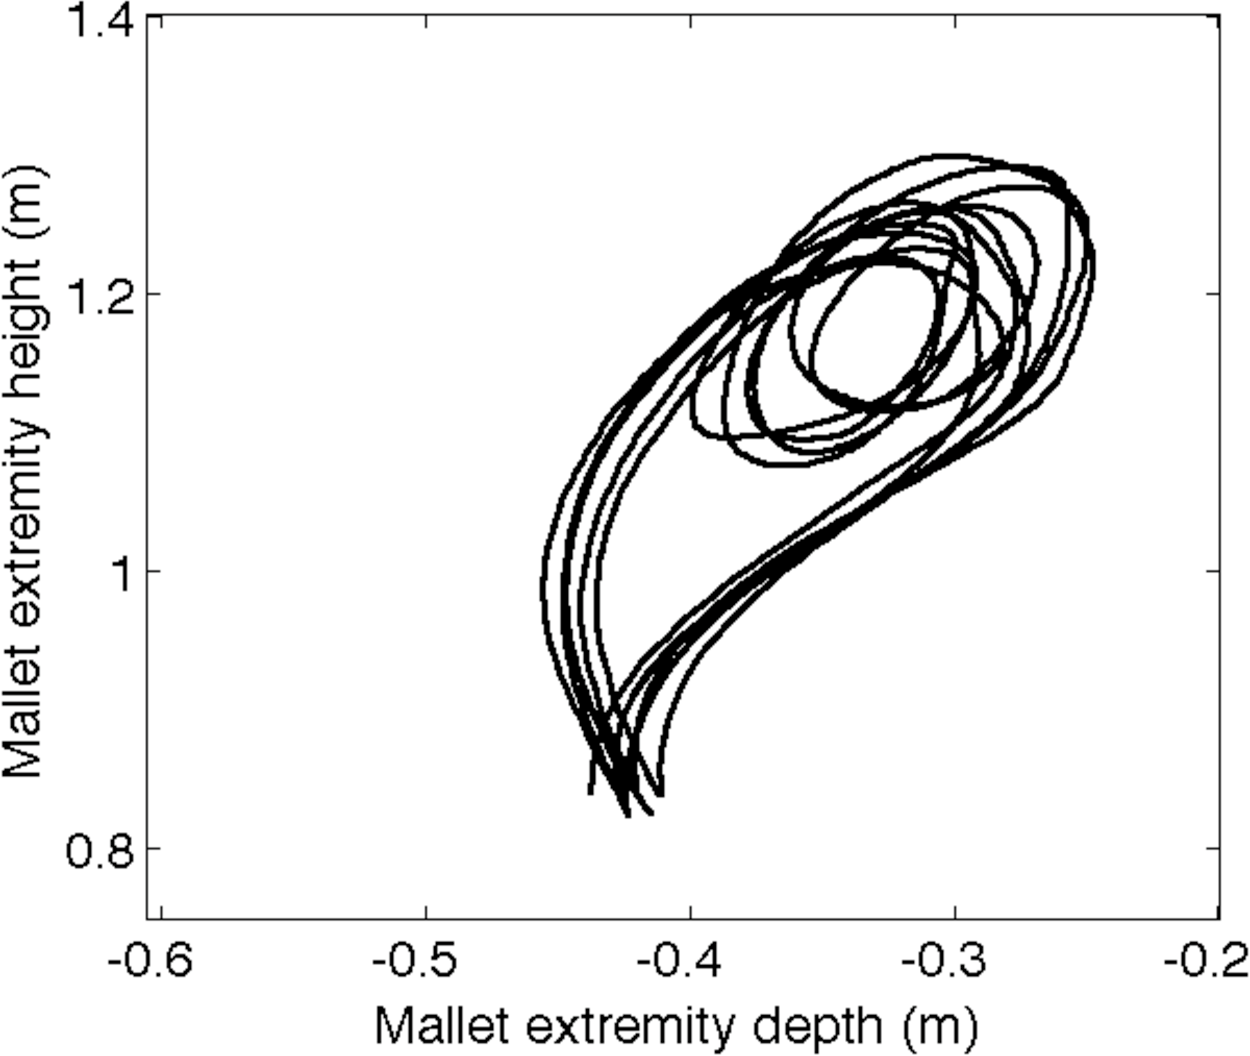
\includegraphics[width=0.45\linewidth]{Chapters/4/Pics/Pdf/legato.pdf}}
		\hspace{6mm}
		\subfigure[]{\label{fig:playingMode2}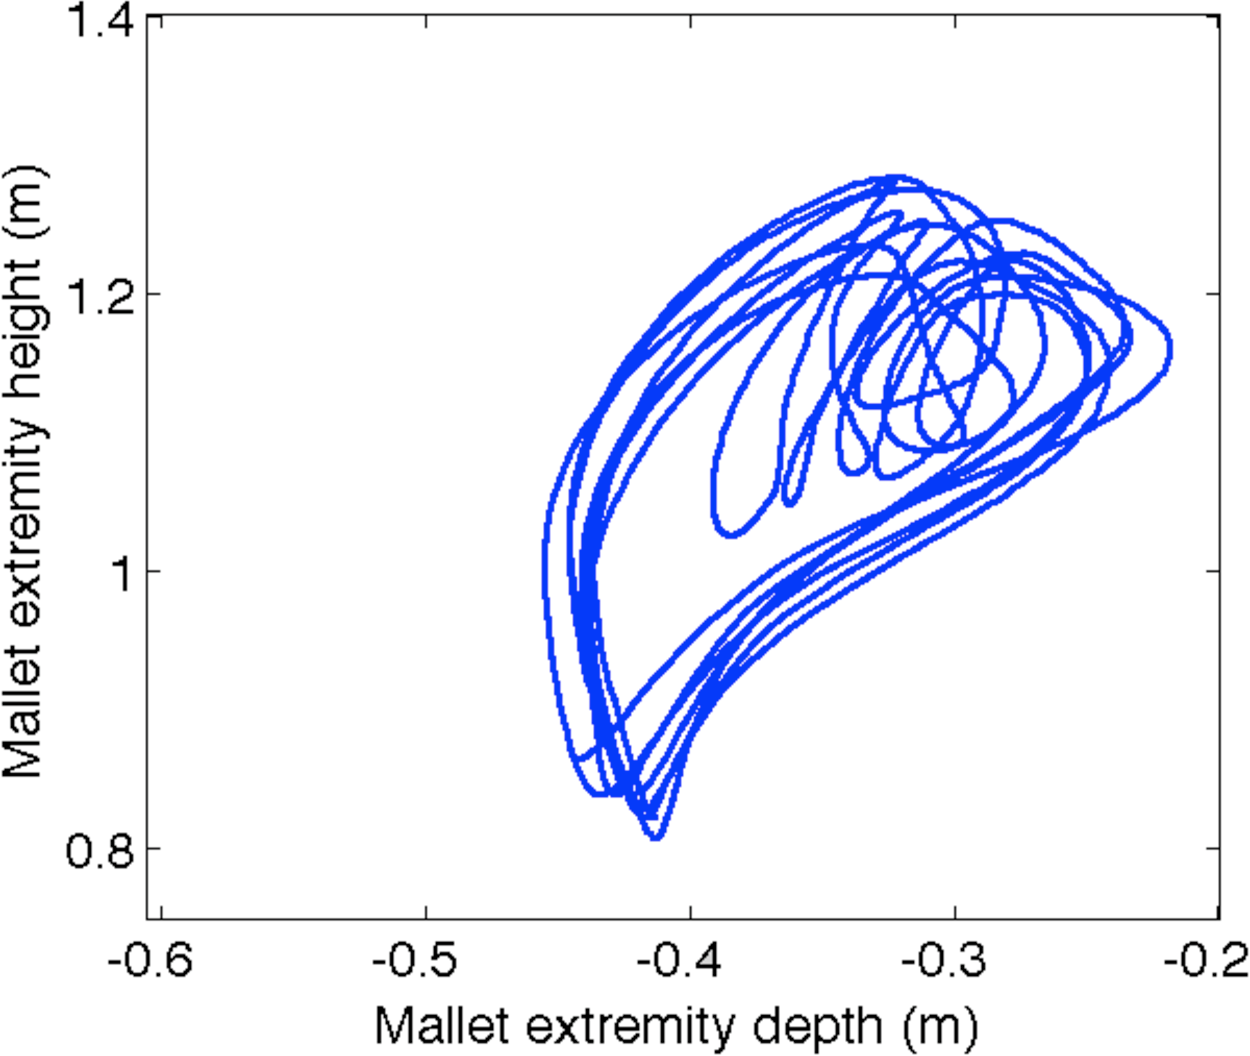
\includegraphics[width=0.45\linewidth]{Chapters/4/Pics/Pdf/tenuto.pdf}}\\
		\subfigure[]{\label{fig:playingMode3}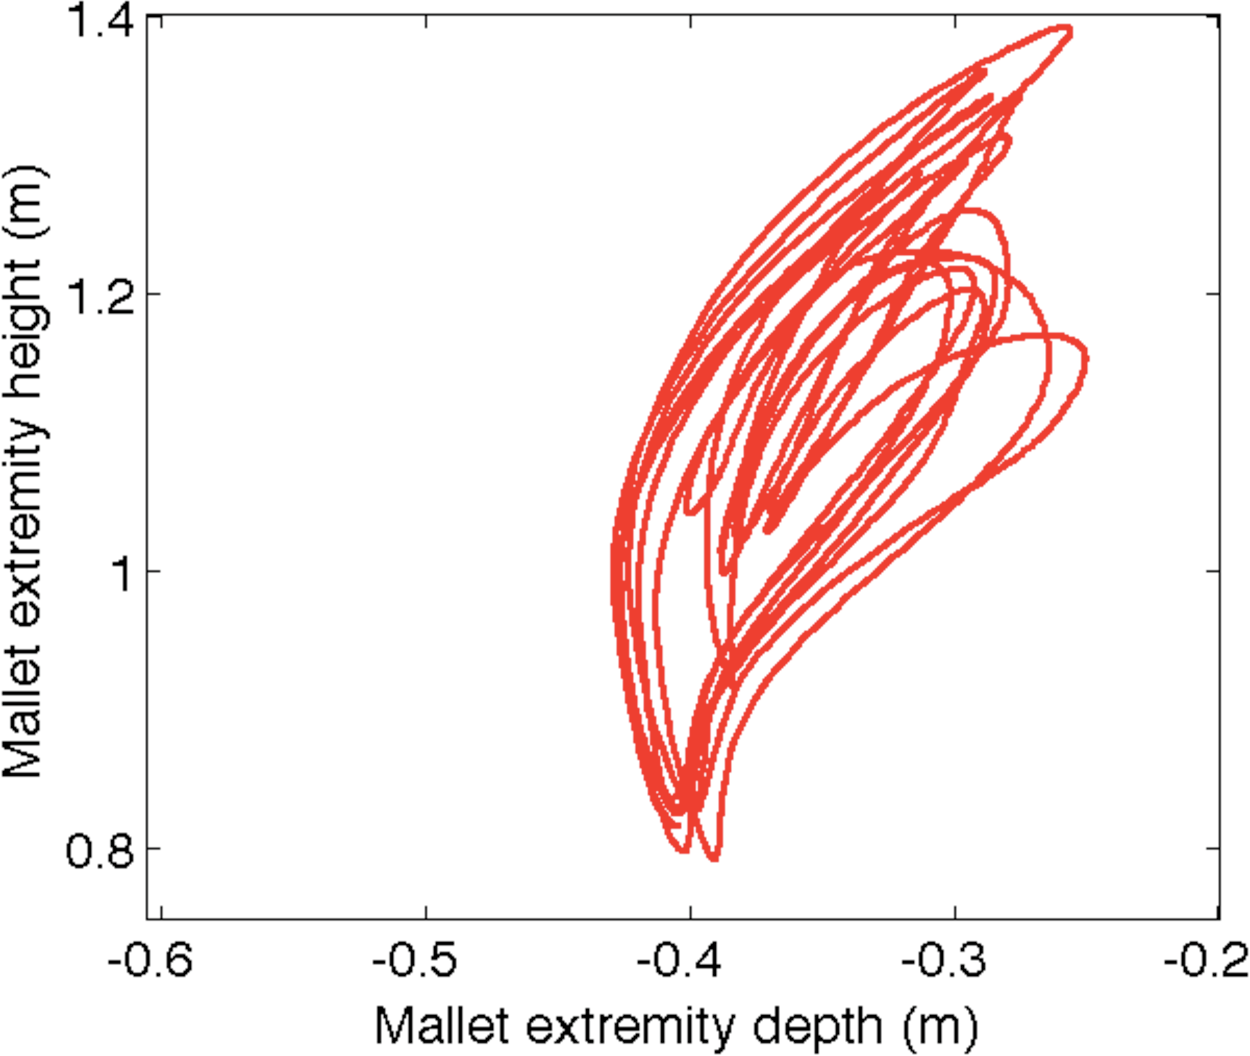
\includegraphics[width=0.45\linewidth]{Chapters/4/Pics/Pdf/accent.pdf}}
		\hspace{6mm}
		\subfigure[]{\label{fig:playingMode4}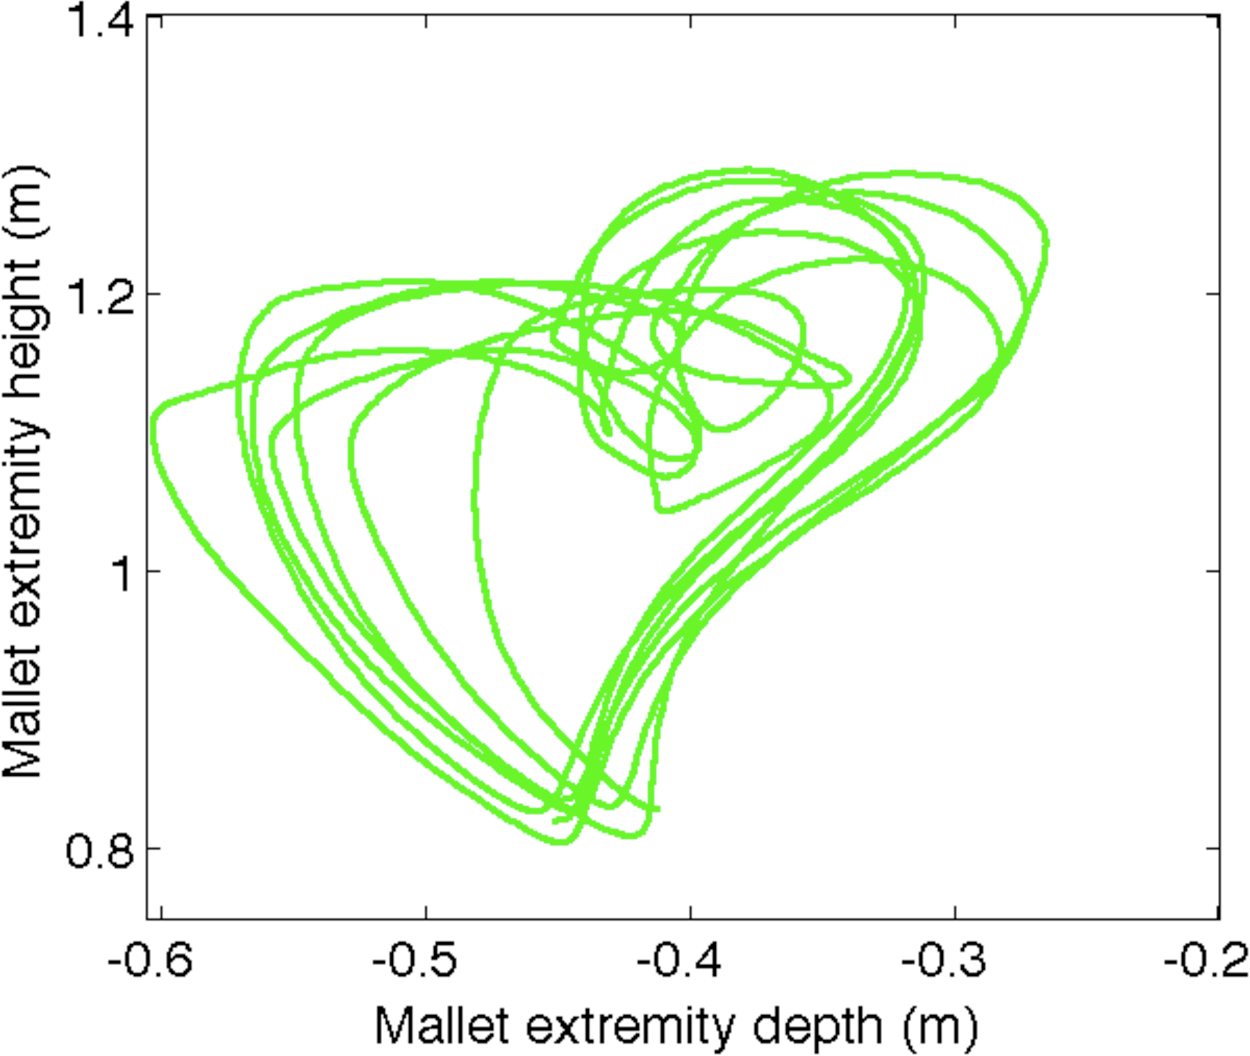
\includegraphics[width=0.45\linewidth]{Chapters/4/Pics/Pdf/verticalAccent.pdf}}\\
		\subfigure[]{\label{fig:playingMode5}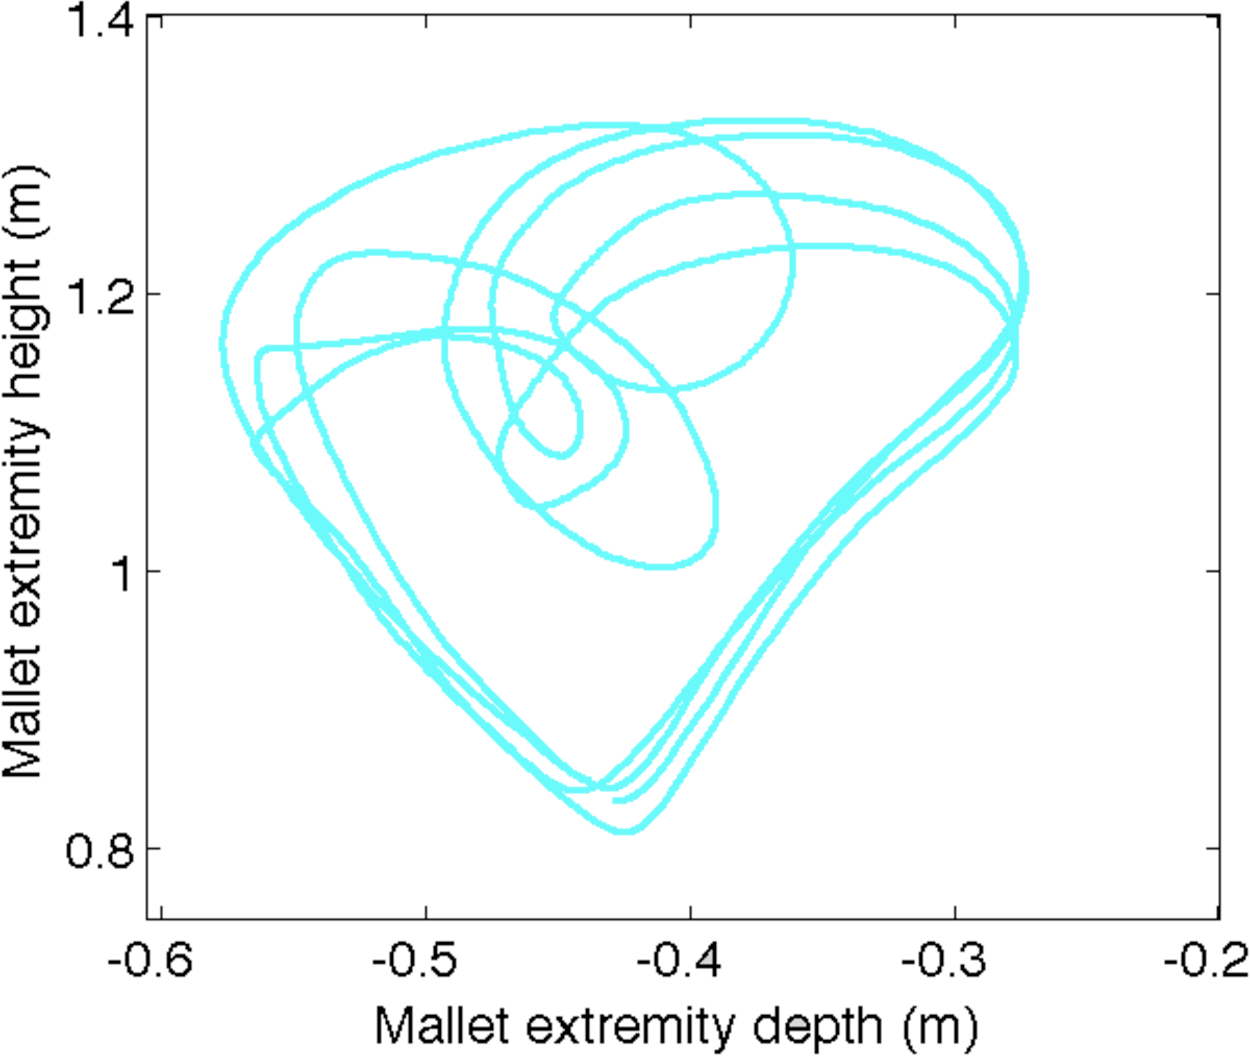
\includegraphics[width=0.45\linewidth]{Chapters/4/Pics/Pdf/staccato.pdf}}
	\end{center}
	\vspace{-0.6cm}
	\caption[Playing modes]{Mallet extremity trajectories in the sagital plane for the various playing modes: (a) \emph{legato}, (b) \emph{tenuto}, (c) \emph{accent}, (d) \emph{vertical accent}, (e) \emph{staccato}. The same color typology will be used further for representing these playing modes.}
	\label{fig:playingModes}
\end{figure}

Various playing modes can also been identified in timpani percussion performances. This includes different gesture variations, such as \emph{legato}, \emph{tenuto}, \emph{accent}, \emph{vertical accent} and \emph{staccato}. \myfigname \ref{fig:playingModes} depicts examples of these playing modes for the \emph{French} grip, through different profiles of mallet trajectories in the sagital plane.

A first observation leads to the identification of "air-beats" between two beat attacks, characterized by internal "loops" in the curves. These air-beats can be interpreted as a strategy from performers for keeping a regular tempo and counting the number of left and right beat attacks. It should be noted that these air-beats may not be present for recorded data at a higher tempo.

These playing modes show also different gesture dynamics, both in the longitudinal and vertical directions. While \emph{legato} and \emph{tenuto} playing modes are quite similar, \emph{accent} show a more stiff movement characterized by a bigger vertical amplitude, a lower longitudinal displacement, and therefore more constrained air-beats. Moreover, \emph{vertical accent} and \emph{staccato} shows a wider range of motion in the longitudinal direction, especially with a front projection of the mallet during the retractation phase (after the beat impact).\\

At a broader scale, whatever technique the timpanist is using, a compromise is generally found between the combined use of 1) the fingers, 2) the tightness of the grip on the shaft of the mallet, location of the grip on the mallet (depending of the length, diameter of the shaft and weight of the head of the mallet), 3) the position of the hand, 4) the amplitude and speed of the wrist, 5) the amplitude and speed of the forearms and arms, and eventually 6) the possibility or not to change the body's center of gravity (timpanist sitting down or standing up, the second position allowing the performer to use his whole body to control the weight, duration and velocity of the impact). 

%\newpage

%%%%%%%%%%%%%%%%%%%%%%%%%%%%%%%%%%%%%%%%%%%%%%%%%%%%%%%%%%%%%%%%%%%%%%%%%%%%%%%%%%%%%%%%%%%%%%%%%%%%%%%%%%%%%%%%%%%%


%%%%%%%%%%%%%%%%%%%%%%%%%%%%%%%%%%%%%%%%%%%%%%%%%%%%%%%%%%%%%%%%%%%%%%%%%%%%%%%%%%%%%%%%%%%%%%%%%%%%%%%%%%%%%%%%%%%%

	\section{Motion Capture Protocol and Database}
	\label{sec:Analysis_MoCapDatabase}


%		\subsection{Global Setup}
%		\label{subsec:Analysis_MoCapDatabase_MoCapSetup}

We captured the motion of several timpani performers by using a Vicon 460 system \citeCGA{vicon} based on Infra-Red camera tracking, as well as a standard DV camera that allow both the synchronization and retrieval of gesture and sound. Percussionists used a lycra suit fitted with markers placed according to the marker position of Vicon's \emph{Plug-in Gait}.  In order to retrieve beat impacts, markers have also been placed on the mallets. It should be noted that the placement of markers on mallets can have an impact on the recorded performance since it can slightly change their balance. The balance between left and right mallets can also be altered since different placements have been used, as a mean of recognizing left and right mallets during the post-processing phase of motion data. A careful choice of the size of the timpani has been done as regards to capture conditions. A 23'' timpani has therefore been used in order to minimize the occlusion of markers by the timpani bowl.\\

\begin{figure}%[H]
	\begin{center}
		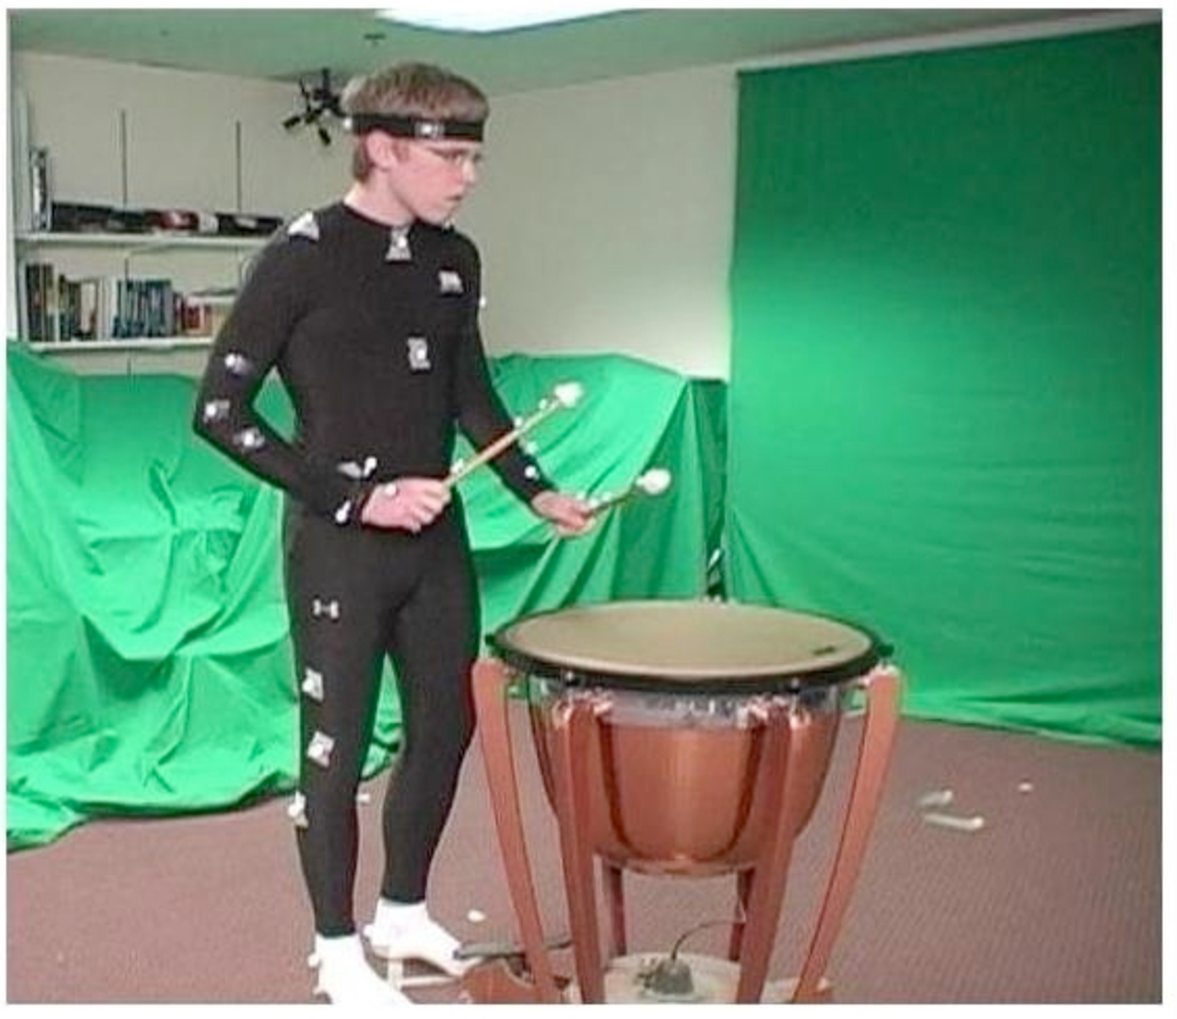
\includegraphics[height=60mm]{Chapters/4/Pics/Pdf/mocapSubject.pdf}
	\end{center}
	\vspace{-0.5cm}
	\caption[Timpani performer and the motion capture setup]{Timpani performer and the motion capture setup.}
	\label{fig:mocapSubject}
\end{figure}

Three percussionists (c.f. \myfigname \ref{fig:mocapSubject}) were asked to perform a pre-defined capture protocol consisting of a single stroke roll for each gesture (\emph{legato}, \emph{tenuto}, \emph{accent}, \emph{vertical accent} and \emph{staccato}). The capture protocol given to performers is provided in appendix \ref{chapter:MoCap}, as well as the corresponding ethical form.

For each gesture, performers were asked to change the location of the beat impact according to the three locations described in subsection \ref{sec:Analysis_TimpaniBasics}. In total, fifteen examples of timpani exercises were performed for each percussionist (each with five beats per hand).

\mytabname \ref{tab:mocapDatabase} presents a summary of the playing characteristics for each performer. The main differences across performers lie in their degree of expertise (\emph{B.A. student}, \emph{M.A. student} or \emph{Prof.}), the grip strategy used (\emph{French} or \emph{German}), their dominant (\emph{Left} or \emph{Right}) hand, and gender.\\

\begin{table}%[H]
	\centering
	\caption[MoCap subjects playing characteristics]{Subjects playing characteristics.}
	\vspace{2mm}
	\begin{tabular}{||x{2cm}||x{2cm}|x{2cm}|x{2cm}|x{2cm}||} \hline
		\small{$Features$ / $Subject$} & \small{$Expertise$} & \small{$Grip$} & \small{$Hand$} & \small{$Gender$} \tabularnewline \hline \hline
		\small{$S_1$} & \small{Prof.} 	& \small{French} 	& \small{Right} 	& \small{M} \tabularnewline \hline
		\small{$S_2$} & \small{B.A.}	& \small{German} 	& \small{Left}	 	& \small{M} \tabularnewline \hline
		\small{$S_3$} & \small{M.A.}	& \small{German} 	& \small{Right} 	& \small{F} \tabularnewline \hline
	\end{tabular}
	\label{tab:mocapDatabase}
\end{table}


%		\subsection{Choice of Sampling Rate}
%		\label{subsec:Analysis_MoCapDatabase_SamplingRate}

One of the main issues using such hardware solutions is the choice of the sampling rate used for the capture of percussive gestures (because of the short duration of the beat impact \citeIPA{dahl97, wagner:MsC06}).

With a high sampling rate (500 Hz and above), one can expect to more accurately retrieve beat attacks, but the spatial range is significantly reduced so that it may be difficult to capture the whole body of the performer.  For this project, a compromise was chosen by setting the cameras at 250 Hz, allowing both full-body capture as well as a reasonably high sampling rate for capturing reliably mallet beat impacts. 


%		\subsection{Motion Database Refinement: Segmentation}
%		\label{subsec:Analysis_MoCapDatabase_Segmentation}

%%%%%%%%%%%%%%%%%%%%%%%%%%%%%%%%%%%%%%%%%%%%%%%%%%%%%%%%%%%%%%%%%%%%%%%%%%%%%%%%%%%%%%%%%%%%%%%%%%%%%%%%%%%%%%%%%%%%


%%%%%%%%%%%%%%%%%%%%%%%%%%%%%%%%%%%%%%%%%%%%%%%%%%%%%%%%%%%%%%%%%%%%%%%%%%%%%%%%%%%%%%%%%%%%%%%%%%%%%%%%%%%%%%%%%%%%

	\section{Analysis}
	\label{sec:Analysis_TimpaniAnalysis}

We present here the analysis of timpani performance gestures collected in our database. This analysis focuses on the study of the trace of the percussionist action during musical performance: mallet extremity trajectories. As it can be intuitively stated \citeIPA{bouenard:ENACTIVE08}, percussionists more specifically control the motion of mallets over time. The aim of the following analysis is to provide a quantitative analysis of this hypothesis, as well as giving relevant parameters that are of particular interest for the modeling and synthesis part of our work (chapter \ref{chapter:Synthesis}). In order to highlight this assumption, we conduct below a study which aims at putting in evidence the effect of grips and playing modes on preparatory trajectories of mallet extremity.


		\subsection{Segmentation of Motion Capture Data}
		\label{subsec:Analysis_TimpaniAnalysis_Segmentation}

A refinement to the raw data contained in the motion capture database has been achieved as a first step of analyzing the effect of grips and playing modes on timpani preparatory gestures. As originally underlined in \citeCM{gibet:PhD87, ramstein:PhD91}, these gestural units may be obtained by the physical activity of the performer-instrument interaction (in our case beat impacts during percussion performances). We segment each percussion sequence that has been initially recorded into \emph{beat-to-beat} gesture units. These latter have been identified by processing a detection of beat impacts on mallet height trajectories. \myfigname \ref{fig:beatDetection} depicts a semi-automatic process for, firstly detecting local extrema on mallet trajectories that are potentially beat impacts, and secondly select manually the points of interest. Once \emph{beat-to-beat} gesture units are available for the playing techniques under study (grips and playing modes), it is possible to conduct a fine analysis of the effect of the playing techniques on mallet trajectories.

\begin{figure}%[H]
	\begin{center}
		\subfigure[]{\label{fig:beatDetection1}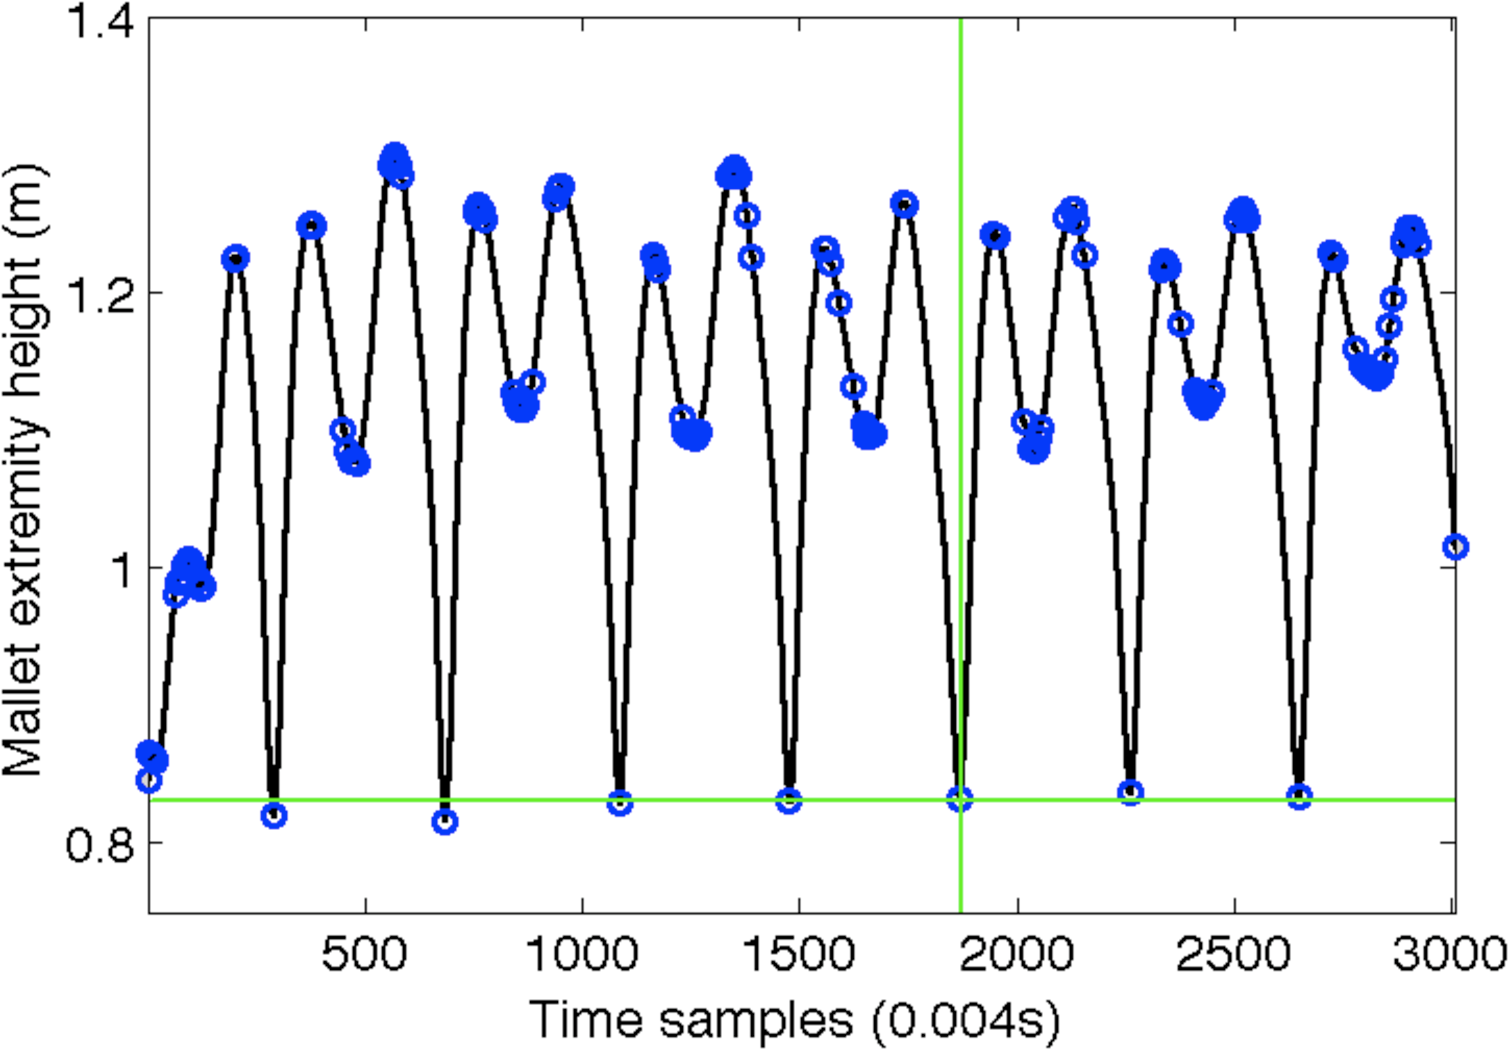
\includegraphics[width=0.495\linewidth]{Chapters/4/Pics/Pdf/beatDetection.pdf}}
		\subfigure[]{\label{fig:beatDetection2}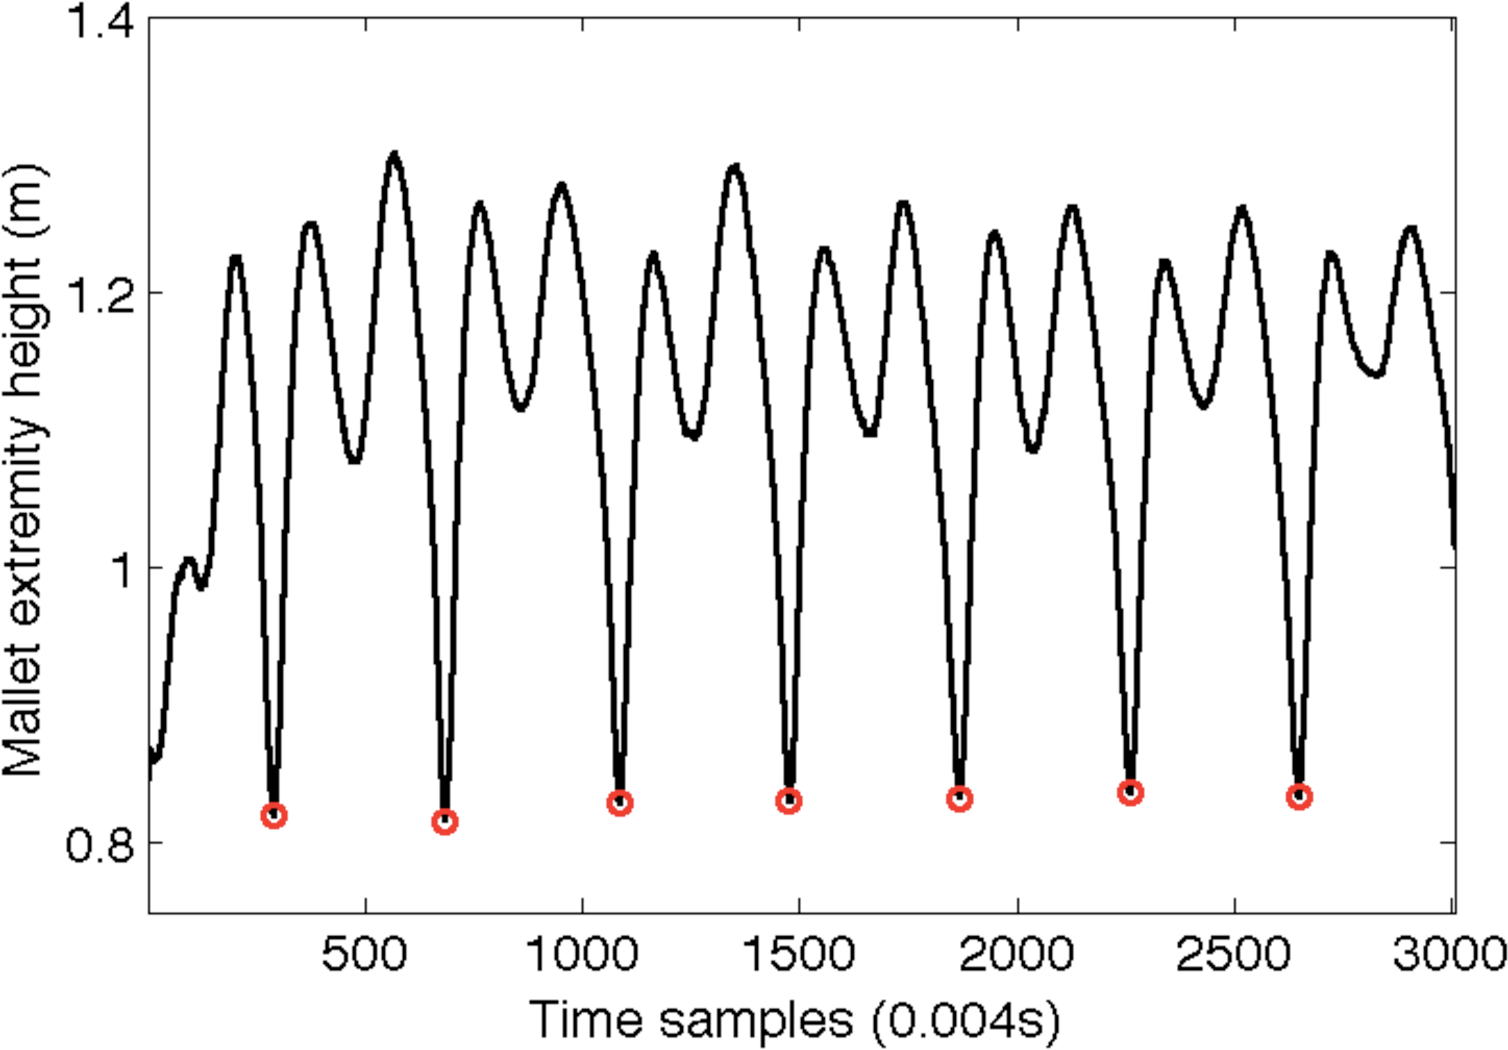
\includegraphics[width=0.495\linewidth]{Chapters/4/Pics/Pdf/beatDetection2.pdf}}
%		\subfigure[]{\label{fig:beatDetection1}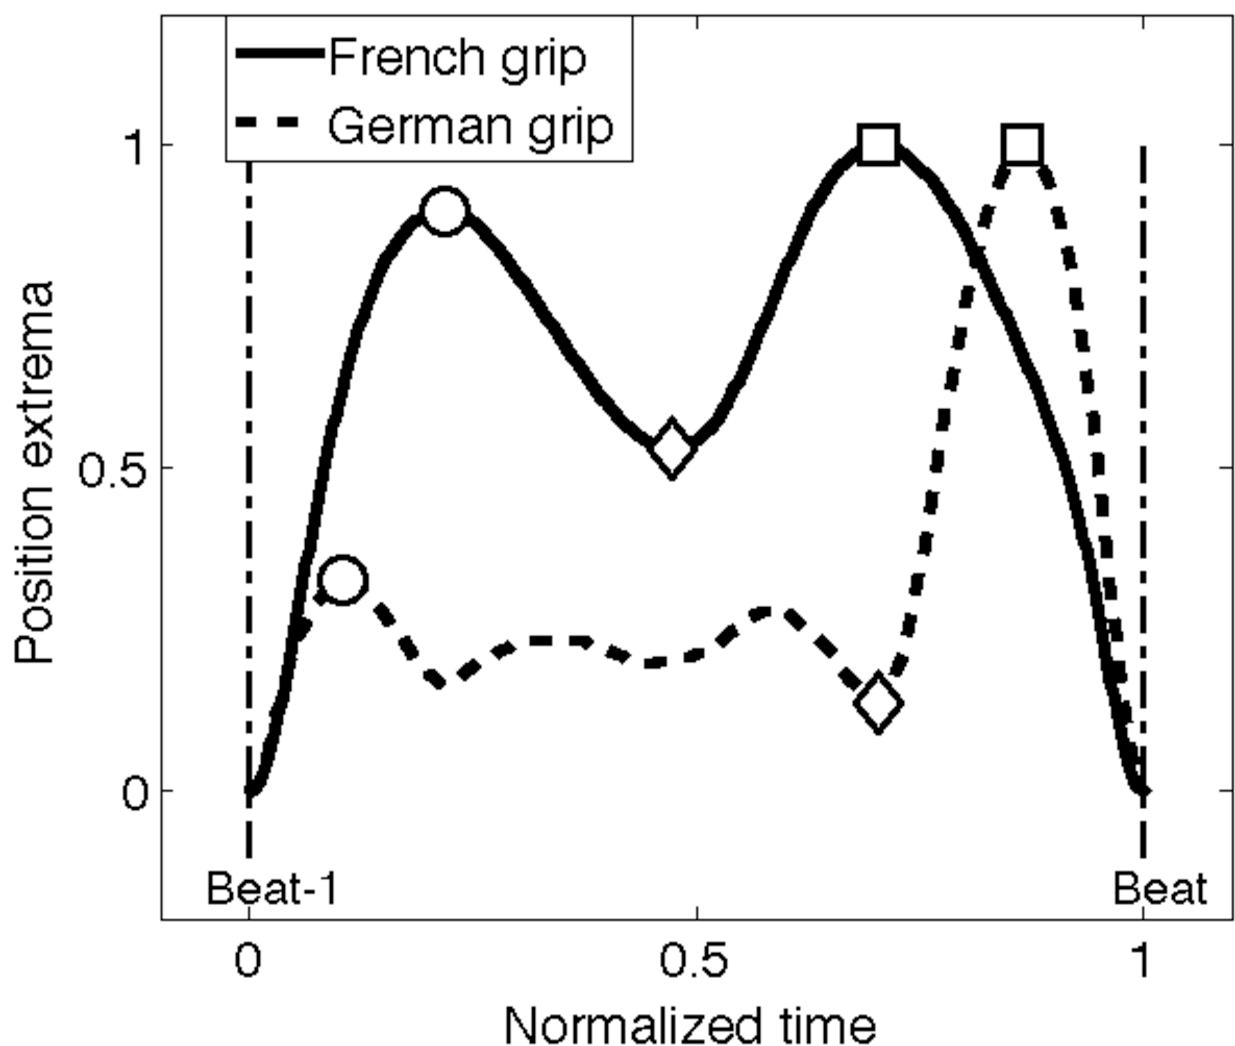
\includegraphics[width=0.45\linewidth]{Chapters/4/Pics/Pdf/pos_parameters.pdf}}
%		\hspace{6mm}
%		\subfigure[]{\label{fig:beatDetection2}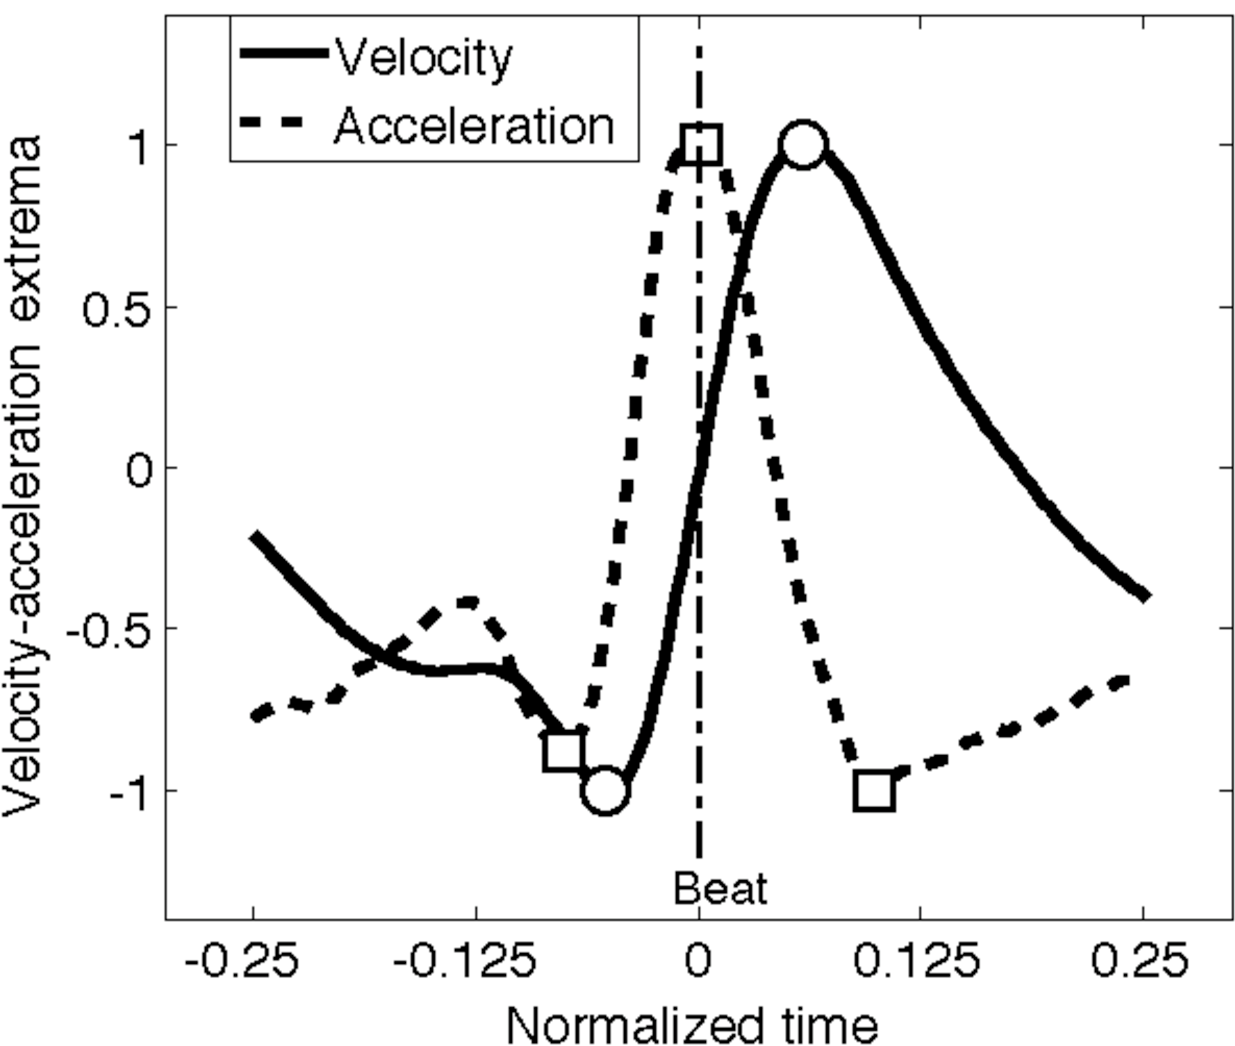
\includegraphics[width=0.45\linewidth]{Chapters/4/Pics/Pdf/vel_acc_parameters.pdf}}
	\end{center}
	\vspace{-0.6cm}
	\caption[Semi-automatic detection of beat impacts]{Semi-automatic detection of beat impacts: (a) detection of local extrema (blue circles) and selection (green cross) of points of interest, (b) resulting beat impacts (red circles).}
	\label{fig:beatDetection}
\end{figure}
		

		\subsection{Methodology}
		\label{subsec:Analysis_TimpaniAnalysis_Methodo}

The parameters used to characterize mallet trajectories are local extrema extracted from position trajectories during \emph{beat-to-beat preparatory} phases (\myfigname \ref{fig:classifParameters1}), as well as local extrema from velocity and acceleration \emph{beat-centered} profiles (\myfigname \ref{fig:classifParameters2}). Each playing mode for a particular grip is represented by a vector of sixteen dimensions, which correspond to the eight amplitude parameters presented in \myfigname \ref{fig:classifParameters} with their corresponding temporal occurence. These parameters are extracted automatically, therefore building a low-dimension representation of grips and playing modes. \myfigname \ref{fig:profiles} depict examples of position, velocity as well as acceleration trajectories for the various playing modes for both \emph{French} and \emph{German} grips.\\ %One can notice that velocity and acceleration parameters may be useful to distiguish a playing mode from another.\\

The evaluation of such a parameterization is conducted by a quantitative analysis based on a classification/recognition scheme. The relevance of these parameters is measured using the Support Vector Machine (\emph{SVM}) classification method, with the use of Radial Basis Functions (\emph{RBF}) as kernel functions. The scope of this evaluation concerns firstly parameters related to percussion grips (\emph{French} or \emph{German}), and secondly playing modes (\emph{legato}, \emph{tenuto}, \emph{accent}, \emph{vertical accent} and \emph{staccato}). For each case, a combination of parameters is chosen and forms a refined data set of the motion capture database, on which the classification/recognition will work. This refined data set is then divided into two sub-sets, an exerpt of it is randomly extracted to represent determined classes that train a classifier, whereas the remaining data represent queries submitted to the classifier. The relevance of the selected parameters is then estimated according to their recognition success by the classifier. In this quantitative study, the determined classes to recognize typically correspond to two classes for percussion grips, and five classes for playing modes.

\begin{figure}%[H]
	\begin{center}
%		\subfigure[]{\label{fig:classifParameters1}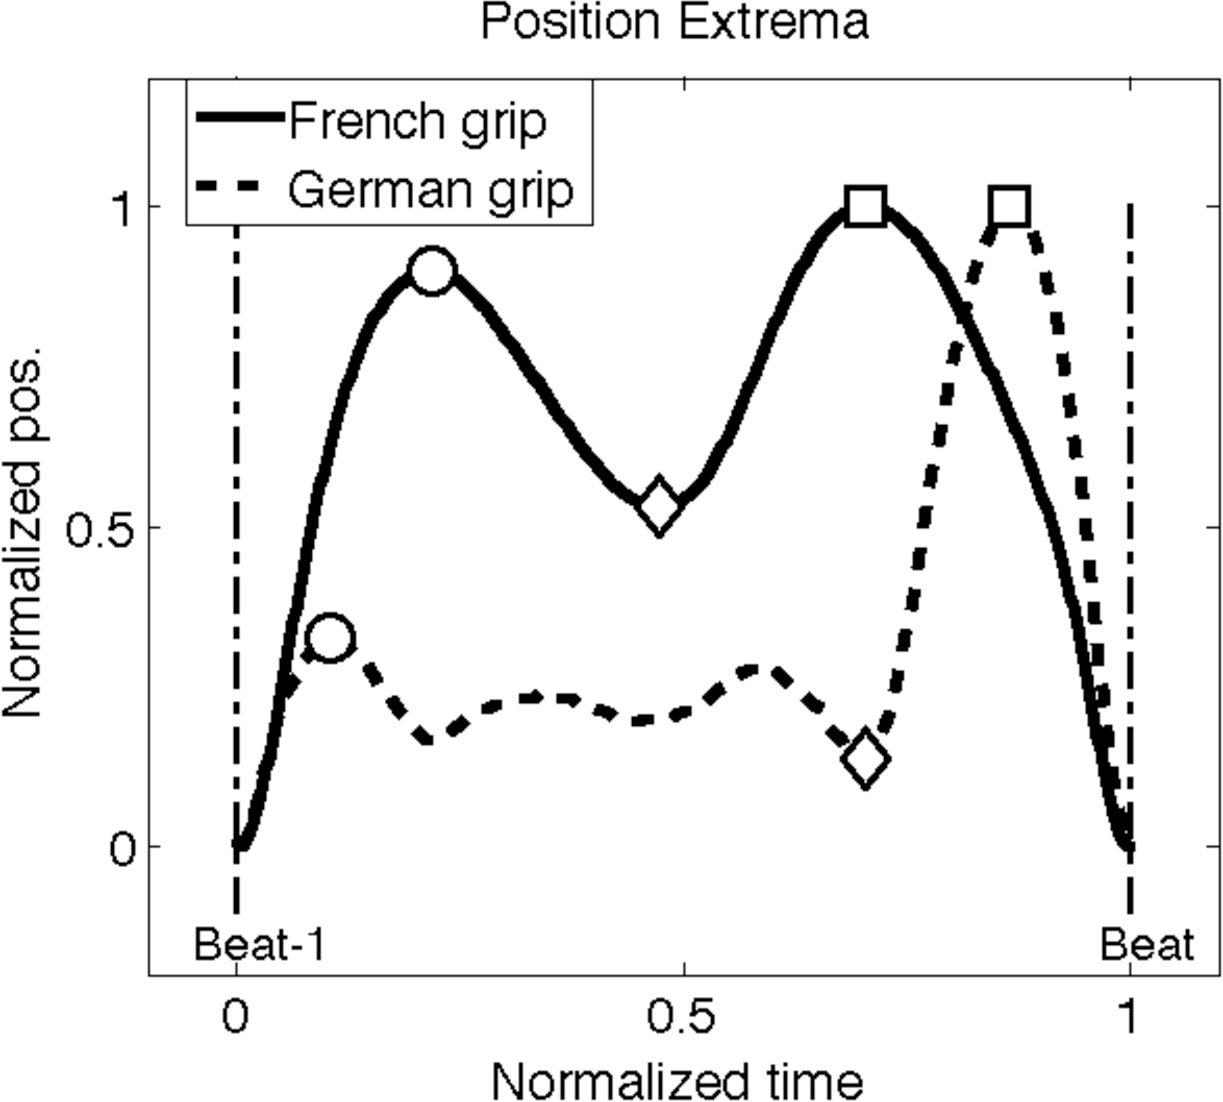
\includegraphics[width=0.45\linewidth]{Chapters/4/Pics/Pdf/GripsProfiles_Normalized2.pdf}}
%		\hspace{6mm}
%		\subfigure[]{\label{fig:classifParameters2}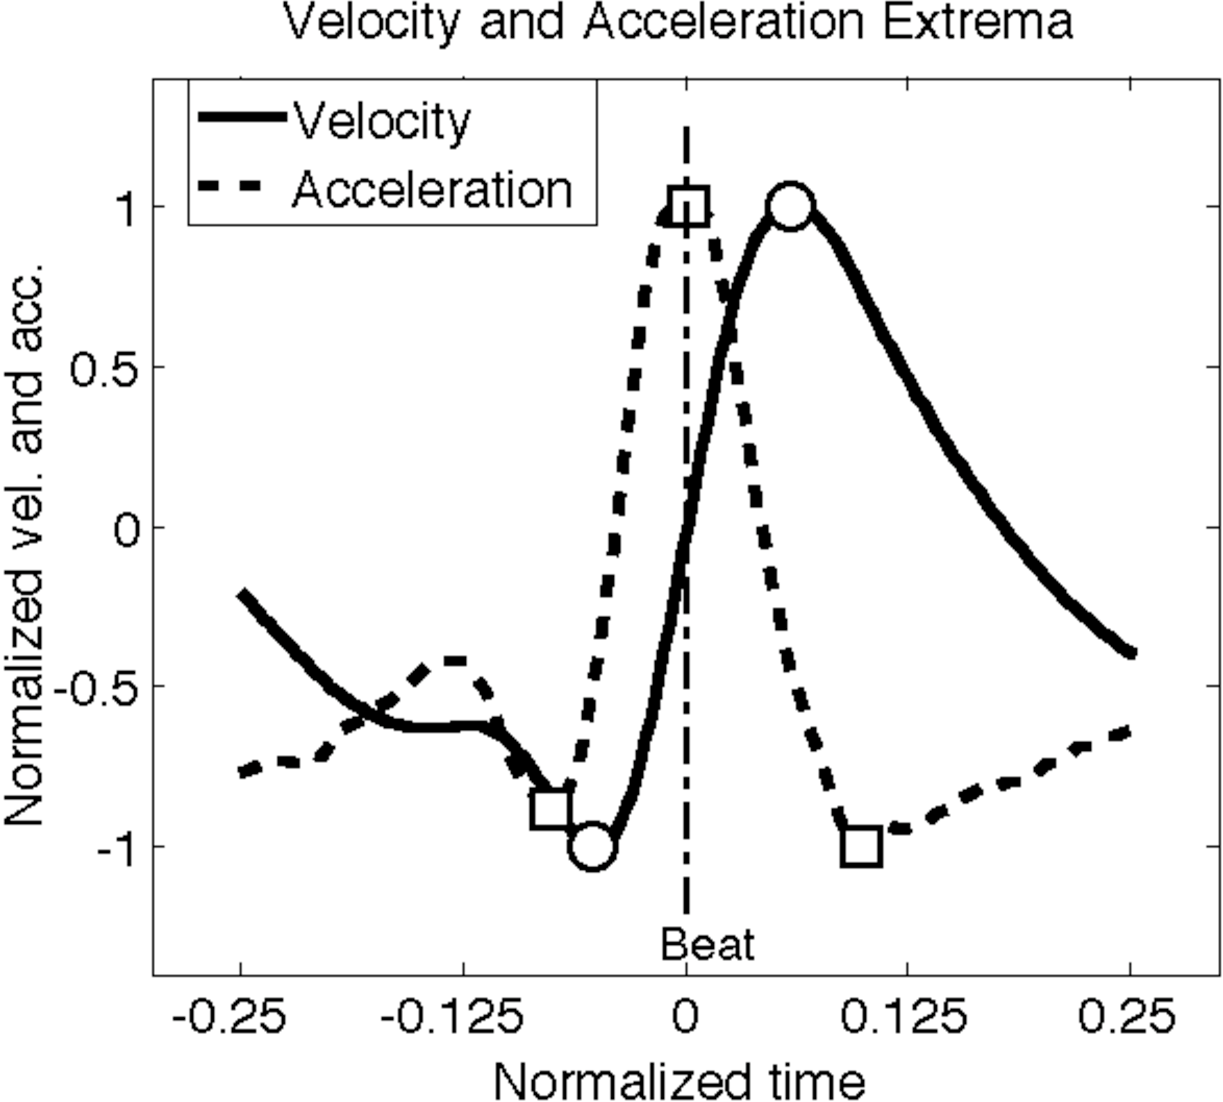
\includegraphics[width=0.45\linewidth]{Chapters/4/Pics/Pdf/VelocityAccelerationProfiles_Normalized2.pdf}}
		\subfigure[]{\label{fig:classifParameters1}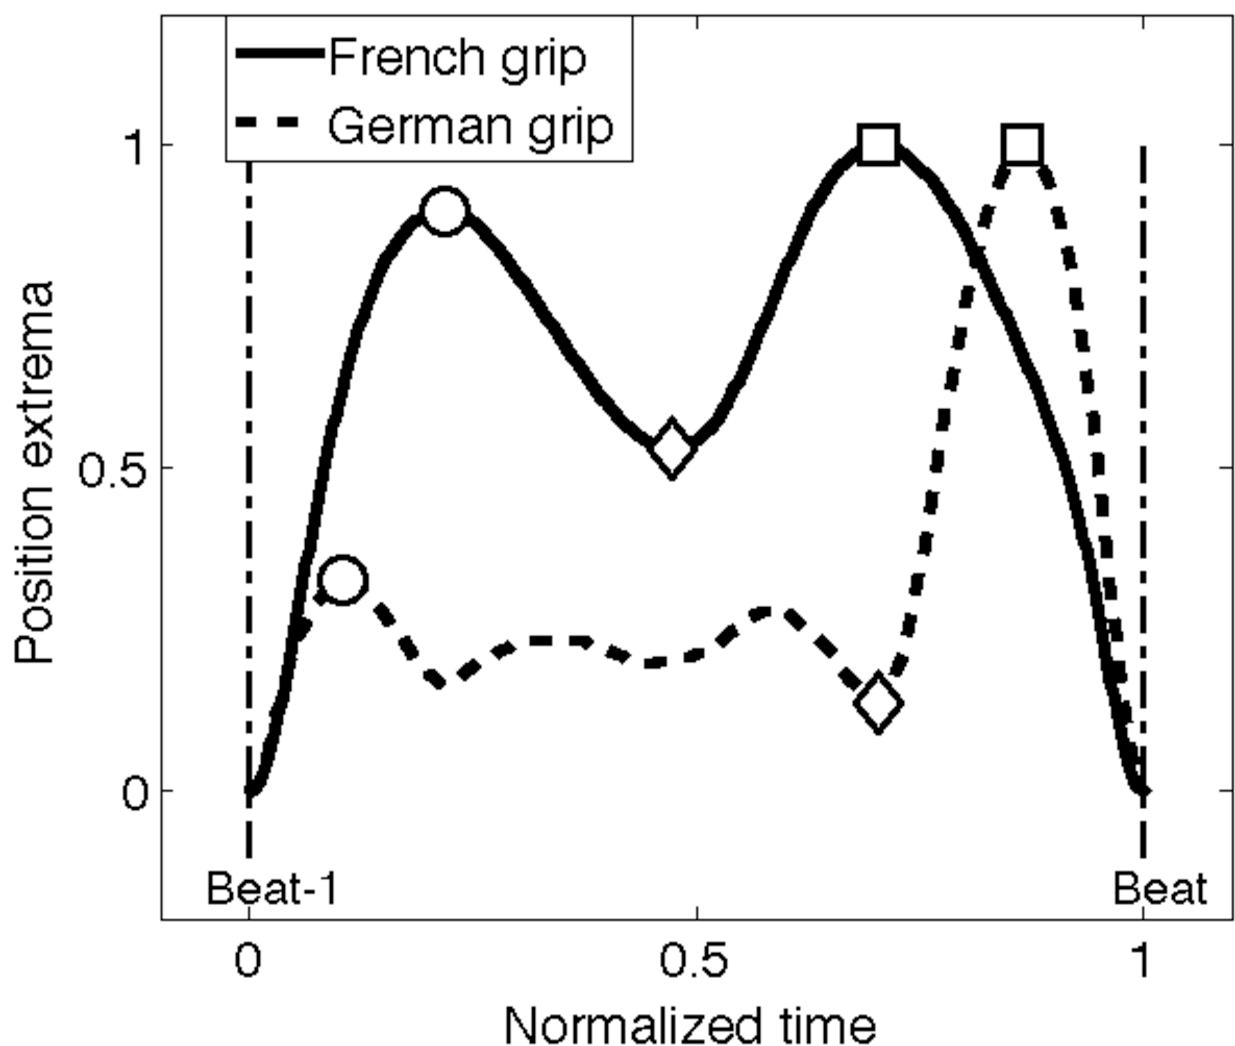
\includegraphics[width=0.45\linewidth]{Chapters/4/Pics/Pdf/pos_parameters.pdf}}
		\hspace{6mm}
		\subfigure[]{\label{fig:classifParameters2}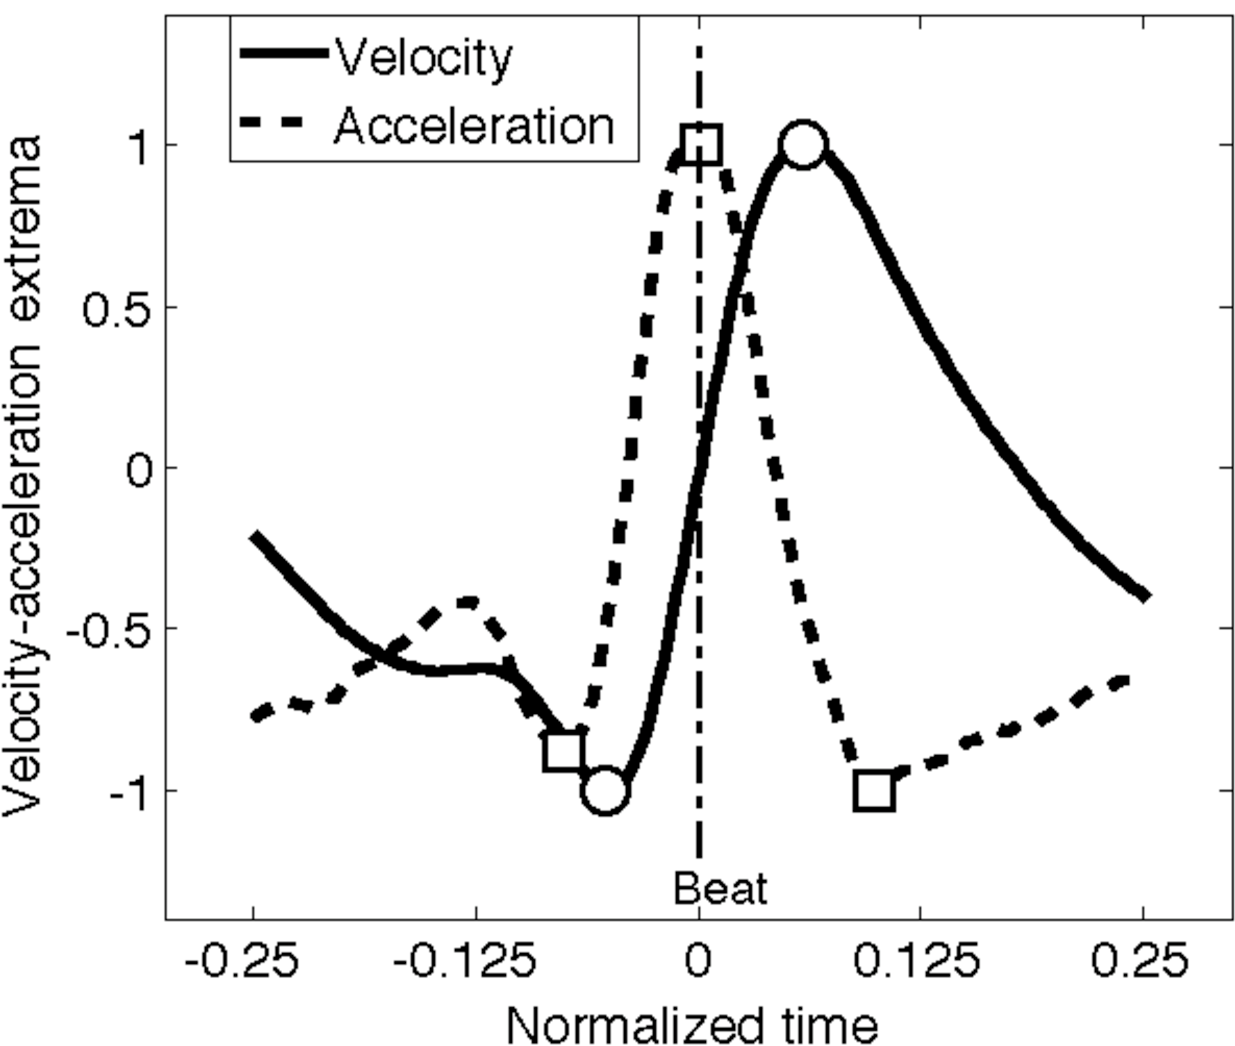
\includegraphics[width=0.45\linewidth]{Chapters/4/Pics/Pdf/vel_acc_parameters.pdf}}
	\end{center}
	\vspace{-0.5cm}
	\caption[Characterization of timpani playing techniques]{Extrema parameters used in the classification/recognition process for characterizing percussion gestures, extracted from: (a) mallet height position during \emph{beat-to-beat preparatory} phases (marker typology: $E_1$ = $\bigcirc$, $E_2$ = $\Diamond$ and $E_3$ = $\square$) and (b) velocity and acceleration \emph{beat-centered} profiles. These parameters are normalized for display purposes.}
	\label{fig:classifParameters}
\end{figure}

\begin{figure}%[H]
	\begin{center}
		\subfigure[]{\label{fig:profiles1}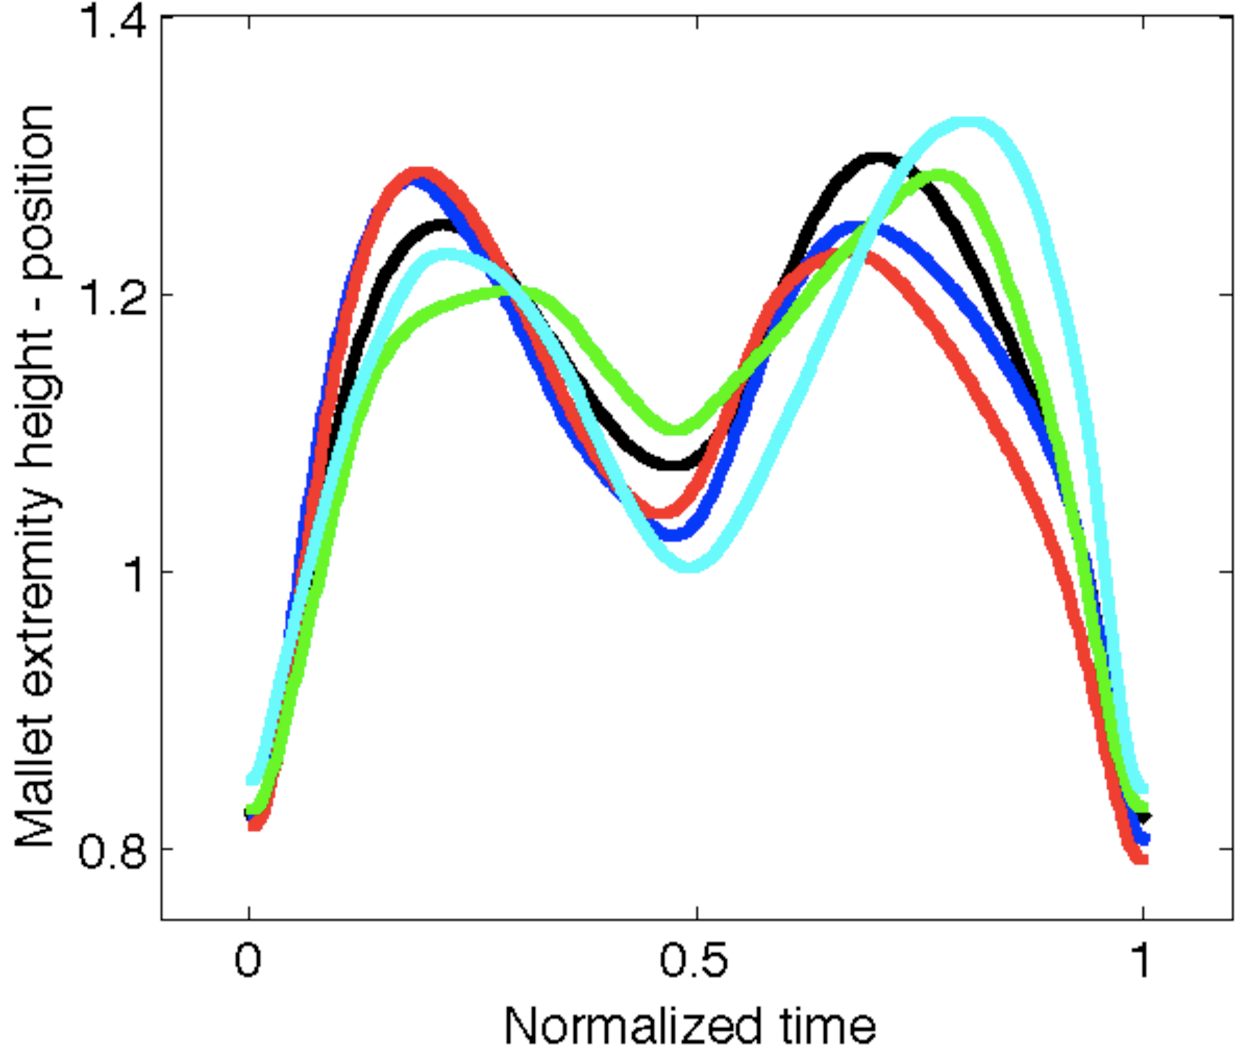
\includegraphics[width=0.45\linewidth]{Chapters/4/Pics/Pdf/french_position.pdf}}
		\hspace{6mm}
		\subfigure[]{\label{fig:profiles2}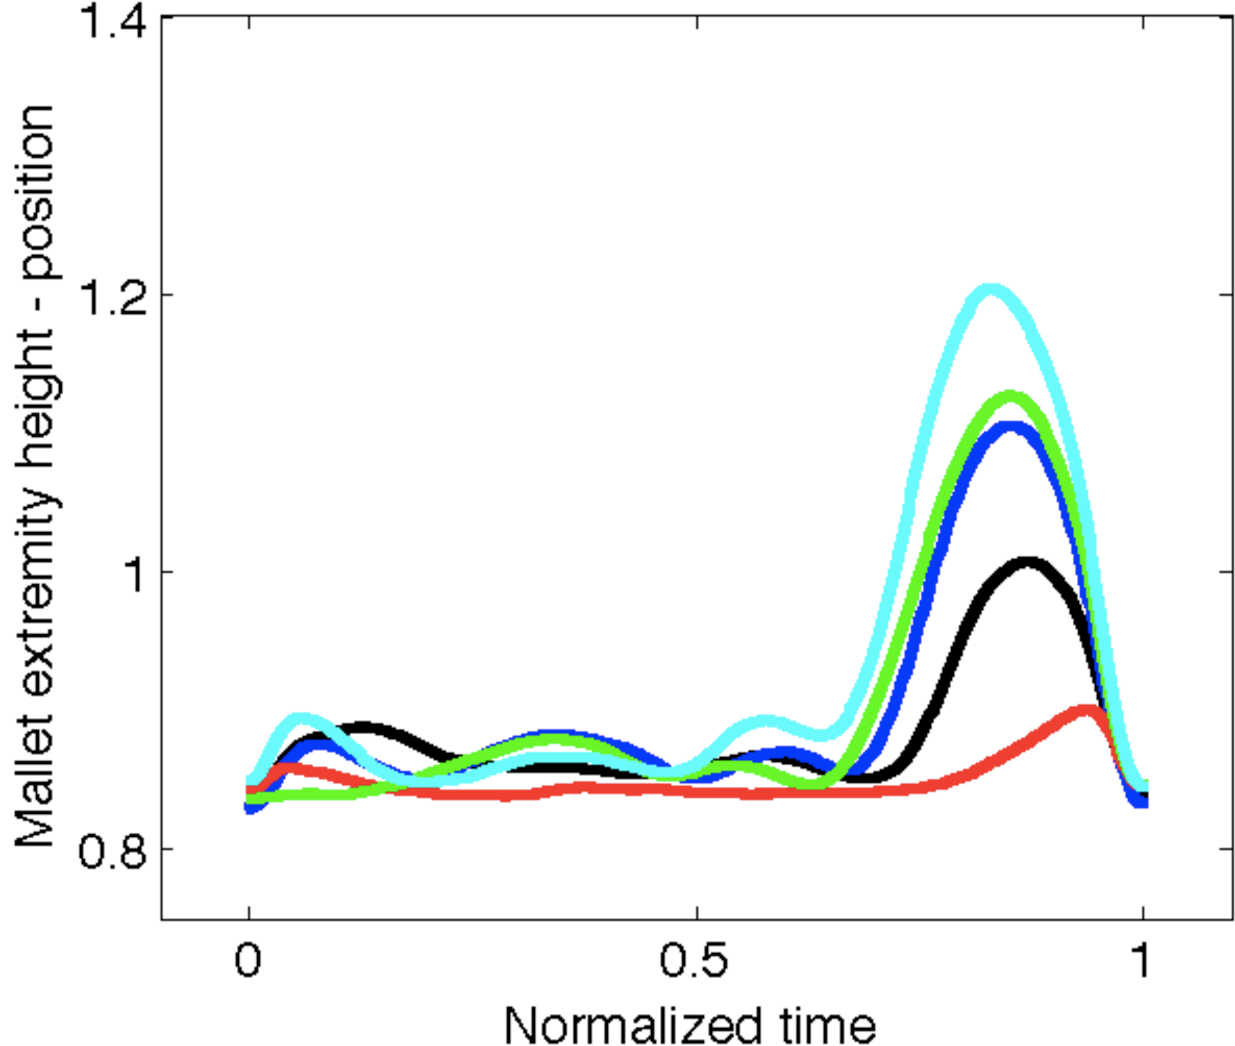
\includegraphics[width=0.45\linewidth]{Chapters/4/Pics/Pdf/german_position.pdf}}\\
		\subfigure[]{\label{fig:profiles3}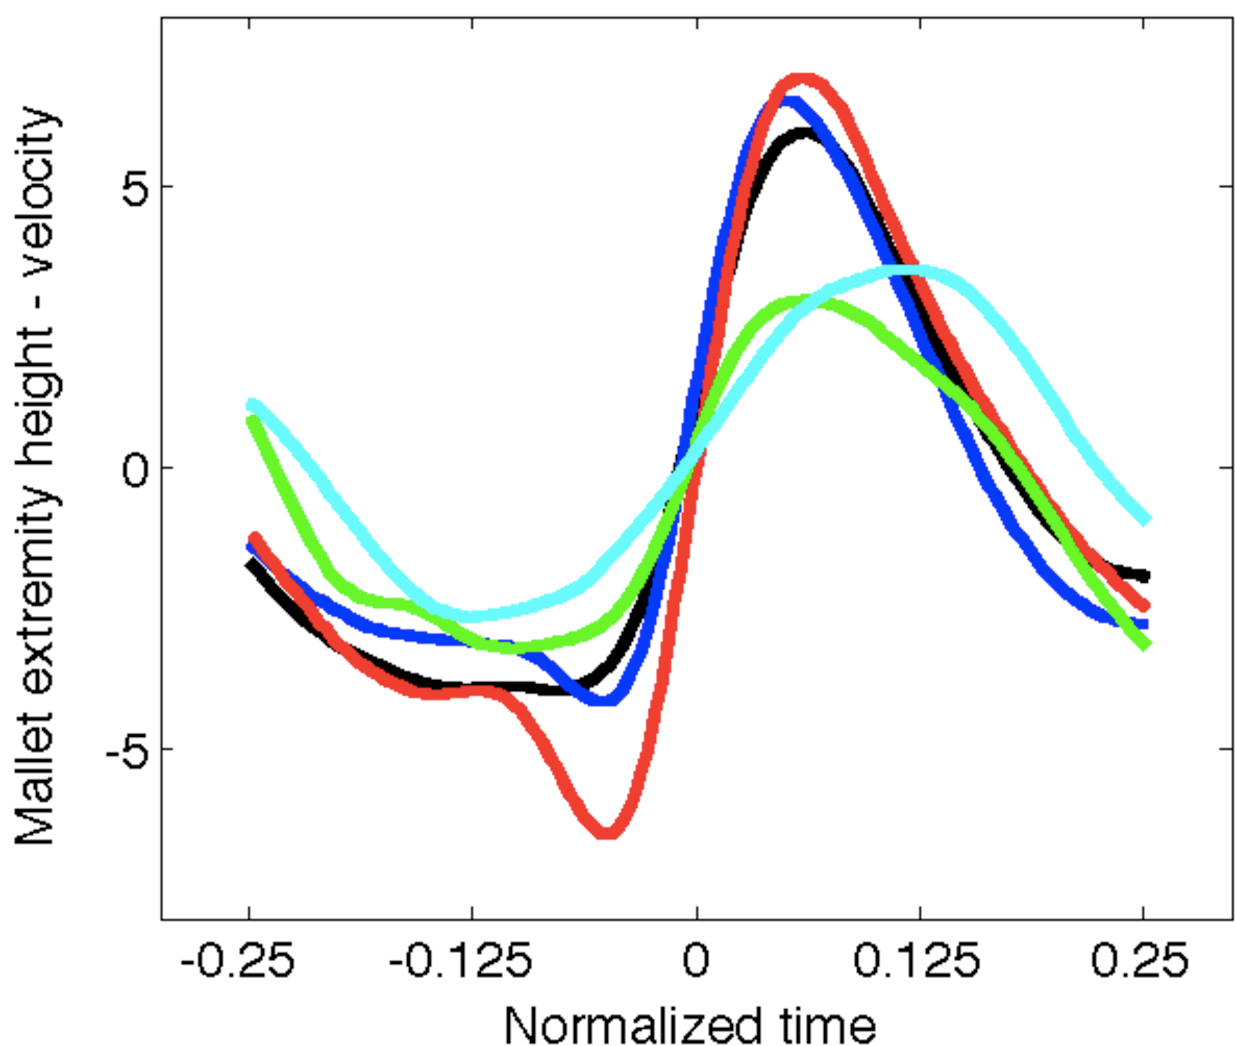
\includegraphics[width=0.45\linewidth]{Chapters/4/Pics/Pdf/french_velocity.pdf}}
		\hspace{6mm}
		\subfigure[]{\label{fig:profiles4}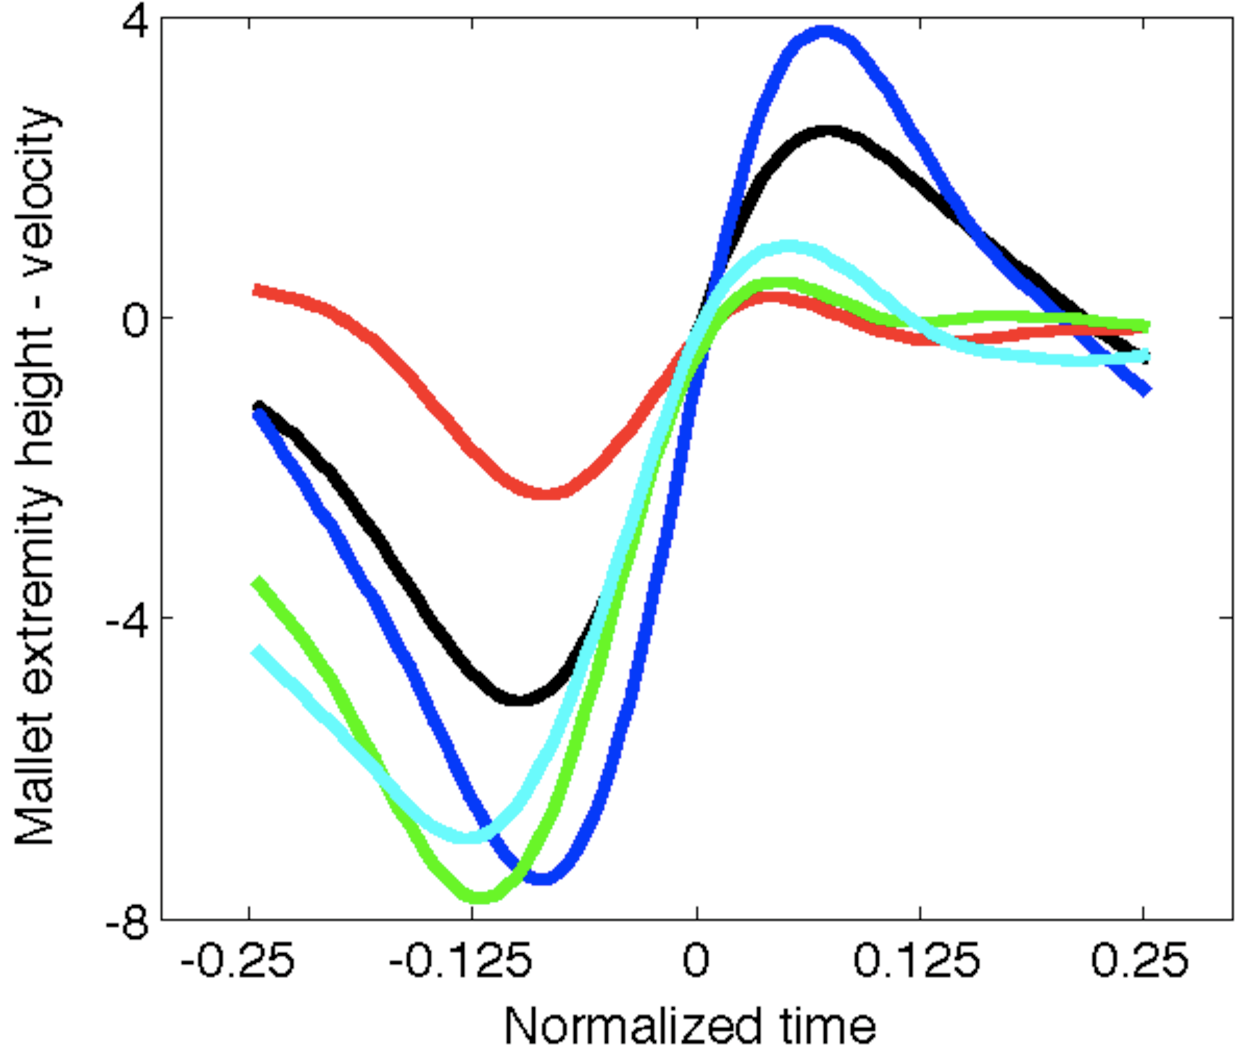
\includegraphics[width=0.45\linewidth]{Chapters/4/Pics/Pdf/german_velocity.pdf}}\\
		\subfigure[]{\label{fig:profiles5}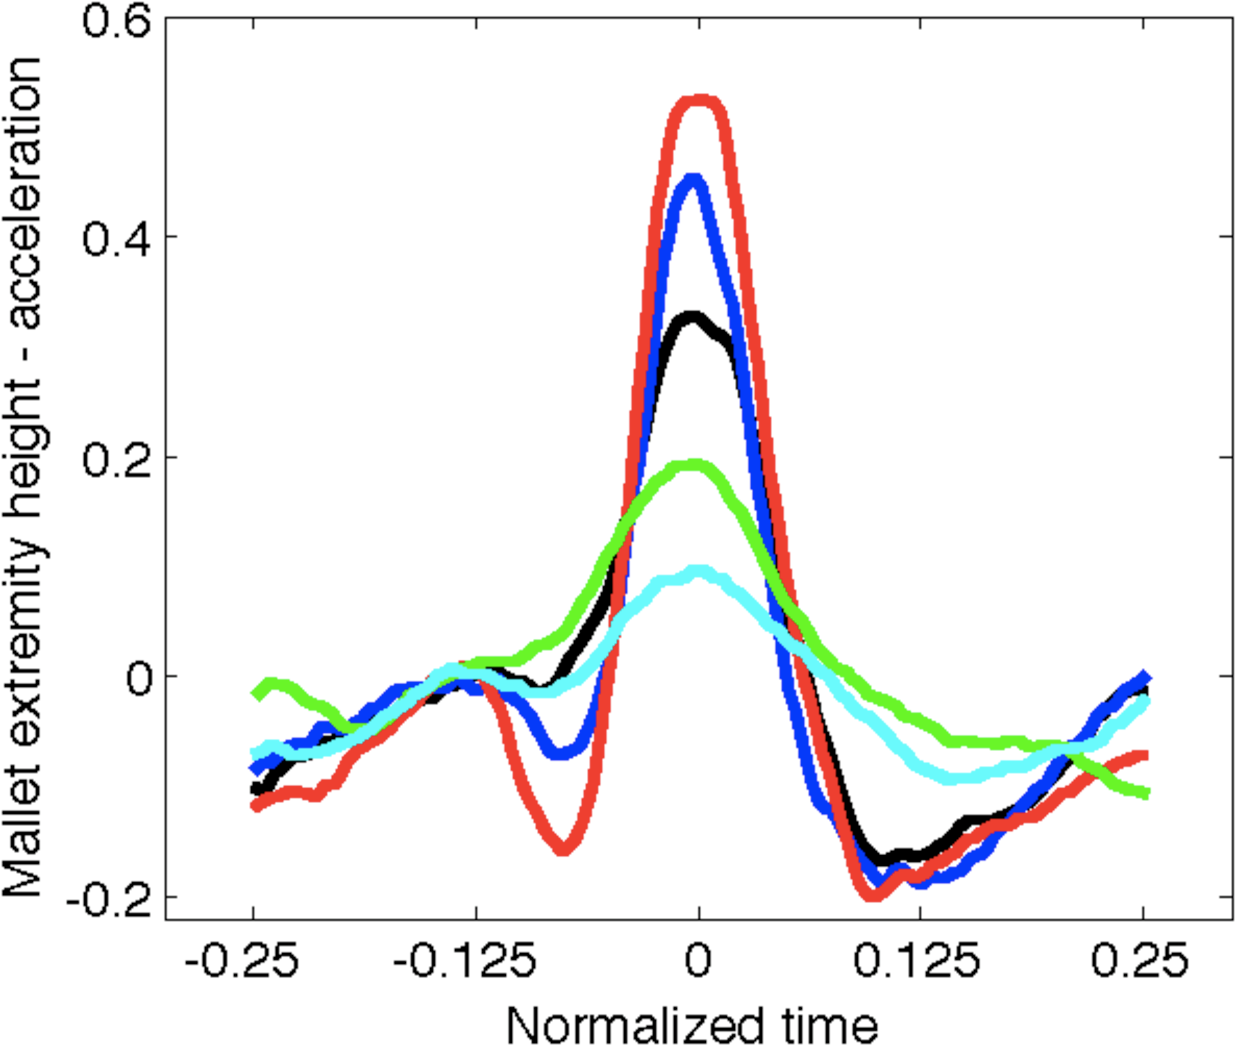
\includegraphics[width=0.45\linewidth]{Chapters/4/Pics/Pdf/french_acceleration.pdf}}
		\hspace{6mm}
		\subfigure[]{\label{fig:profiles6}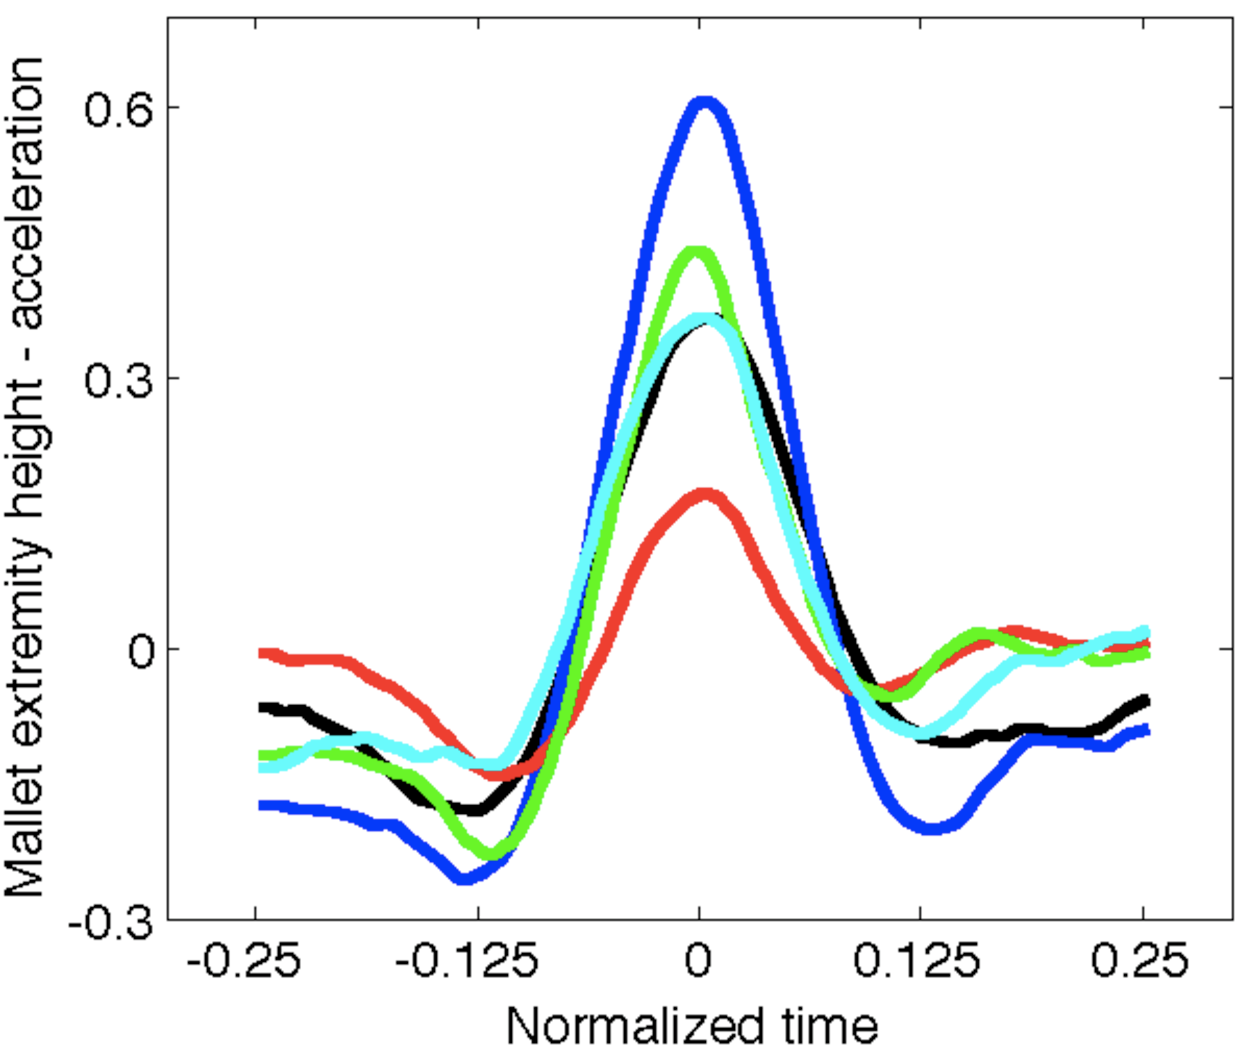
\includegraphics[width=0.45\linewidth]{Chapters/4/Pics/Pdf/german_acceleration.pdf}}
	\end{center}
	\vspace{-0.5cm}
	\caption[Position, velocity and acceleration profiles]{Position, velocity and acceleration profiles, respectively (a), (c) and (e) for the \emph{French} grip, and (b), (d), (f) for the \emph{German} grip.}
	\label{fig:profiles}
\end{figure}


		\subsection{Percussion Grips}
		\label{subsec:Analysis_TimpaniAnalysis_Grips}

First of all, we focus on the analysis of the influence of \emph{French} and \emph{German} grips on mallet trajectories. Quantitative features (\mytabname \ref{tab:statsTip}) processed on the vertical component of the tip of the mallet show that \emph{French} grip-related data performs the same timpani gesture with much more amplitude. The mean of the mallet extremity height is about twenty centimeters higher than its \emph{German} grip counterpart, with a variance twice higher. This fact is strengthened by the vertical range of motion ($RoM$) of the tip of the stick for \emph{French} grip-related data that is about twice higher than for \emph{German} grip data. The mean of mallet extremity height for \emph{German} grip data shows moreover that the tip of the stick is in average closer to the timpani membrane.\\

Specific local extrema can also be observed during the preparatory gesture of beat attacks. \myfigname \ref{fig:classifParameters} presents an example of the vertical component of the preparatory gesture between two beat attacks, and the identification of three characteristic extrema denoted $E_1$, $E_2$ and $E_3$. These extrema are temporally (temporal apparition in percentage of gesture's duration) and spatially characterized in \mytabname \ref{tab:statsTip}.

\begin{table}%[H]
	\centering
	\caption[Mallet trajectories and extracted extrema: statistical features]{Statistical features computed on mallet trajectories and extracted extrema: vertical Mean ($M$), Variance ($Var$) and Range of Motion ($RoM$), as well as the average temporal (in percentage of gesture's duration) and spatial characterization of extracted extrema presented in \myfigname \ref{fig:classifParameters}.}
	\vspace{2mm}
	\begin{tabular}{||x{1.6cm}||x{1.55cm}|x{1.55cm}|x{1.55cm}||x{1.6cm}|x{1.6cm}|x{1.6cm}||} \hline
		\small{$Stats$ / $Grips$} &	\small{$M$} \scriptsize{$[m]$} & 	\small{$Var$} \scriptsize{$[m]$} &	\small{$RoM$} \scriptsize{$[m]$} &	\small{$E_1$} \scriptsize{$[\% / m]$} &	\small{$E_2$} \scriptsize{$[\% / m]$} &	\small{$E_3$} \scriptsize{$[\% / m]$} 			\tabularnewline  \hline \hline
		\small{$French$} &	\small{1.1} &	\small{0.1} &	\small{0.04} &	\small{0.21 / 1.3} &	\small{0.47 / 1.1} &	\small{0.68 / 1.3}	\tabularnewline \hline
		\small{$German$} &	\small{0.9} &	\small{0.05} &	\small{0.02} &	\small{0.12 / 0.9} & 	\small{0.68 / 0.8} &	\small{0.85 / 1.0}		\tabularnewline \hline
	\end{tabular}
	\label{tab:statsTip}
\end{table}

Vertical extrema $E_1$, $E_2$ and $E_3$ are temporally equi-distributed for the \emph{French} grip-related data showing a continuous preparatory gesture, whereas local extrema for \emph{German} grip-related data denote three discontinuous parts. In this latter case, $E_1$ corresponds to the reaction to the previous beat attack, between $E_1$ and $E_2$ the tip of the mallet seems to seek a rest position (during more than the half of the whole movement duration) just above the timpani membrane, while $E_2$ and $E_3$ correspond to the amplitude that \emph{German} grip-related data gives for the following beat attack. \mytabname \ref{tab:statsTip} quantifies also the effect of the \emph{French} and \emph{German} grips on the vertical amplitude of the extrema.\\

\emph{French} and \emph{German} grips influence the spatial and temporal characteristics of the extracted extrema from height trajectories of the tip of the mallets. For evaluating the relevance of such parameters to distinguish these percussion grips, we chose to use a classification/recognition process. The training set is randomly composed of only 1/8$^{th}$ of the total number of available data, and the query set is composed of the remaining data.\\

\begin{table}%[H]
	\centering
	\caption[SVM recognition of timpani grips]{SVM recognition of timpani grips (in percentage of success) using the mallet position extrema presented in \myfigname \ref{fig:classifParameters}.}
	\vspace{2mm}
	\begin{tabular}{||x{1.9cm}||x{1.9cm}|x{1.9cm}||} \hline
		\small{$Training$ / $Test$} & 	\small{$French$} & 		\small{$German$}	\tabularnewline \hline \hline 
		\small{$French$} & 				\small{\textbf{98.2}} & \small{1.8}				\tabularnewline \hline
		\small{$German$} & 				\small{2.7} & 			\small{\textbf{97.3}}	\tabularnewline \hline
	\end{tabular}
	\label{tab:recognitionGrips}
\end{table}

\begin{table}%[H]
	\centering
	\caption[SVM recognition of \emph{French} grip playing modes]{SVM recognition of $French$ grip playing modes (in percentage of success) using the combination of mallet velocity and acceleration extrema presented in \myfigname \ref{fig:classifParameters}.}
	\vspace{2mm}
	\begin{tabular}{||x{1.9cm}||x{1.9cm}|x{1.9cm}|x{1.9cm}|x{1.9cm}|x{1.9cm}||} \hline
		\small{$Training$ / $Test$} & 	\small{$Legato$} &	\small{$Tenuto$} &	\small{$Accent$} &	\small{$V.\ Accent$} &	\small{$Staccato$}\tabularnewline \hline \hline
		\small{$Legato$} & 				\small{\textbf{96.2}} & \small{3.1} & \small{0} & \small{0.7} & \small{0}	\tabularnewline \hline
		\small{$Tenuto$} & 				\small{2.1} & \small{\textbf{92.6}} & \small{3.2} & \small{2.1} & \small{0}	\tabularnewline \hline
		\small{$Accent$} & 				\small{2.4} & \small{0} & \small{\textbf{94.7}} & \small{2.9} & \small{0}	\tabularnewline \hline
		\small{$V.\ Accent$} & 			\small{0} & \small{0} & \small{0} & \small{\textbf{93.4}} & \small{6.6}		\tabularnewline \hline
		\small{$Staccato$} & 			\small{0} & \small{0} & \small{0} & \small{3.3} & \small{\textbf{96.7}}		\tabularnewline \hline
	\end{tabular}
	\label{tab:recognitionFrenchVariations}
\end{table}

\begin{table}%[H]
	\centering
	\caption[SVM recognition of \emph{German} grip playing modes]{SVM recognition of $German$ grip playing modes (in percentage of success) using the combination of mallet position and acceleration extrema presented in \myfigname \ref{fig:classifParameters}.}
	\vspace{2mm}
	\begin{tabular}{||x{1.9cm}||x{1.9cm}|x{1.9cm}|x{1.9cm}|x{1.9cm}|x{1.9cm}||} \hline
		\small{$Training$ / $Test$} & 	\small{$Legato$} & 	\small{$Tenuto$} & 	\small{$Accent$} & 	\small{$V.\ Accent$} & 	\small{$Staccato$}\tabularnewline \hline \hline
		\small{$Legato$} & 				\small{\textbf{92.4}} &	\small{5.1} & \small{0} & \small{2.5} &	\small{0}	\tabularnewline \hline
		\small{$Tenuto$} & 				\small{3.3} & \small{\textbf{93.1}} & \small{0} & \small{1.1} &	\small{2.5}	\tabularnewline \hline
		\small{$Accent$} & 				\small{2.9} & \small{0} & \small{\textbf{94.3}} & \small{2.8} & \small{0}	\tabularnewline \hline
		\small{$V.\ Accent$} & 			\small{1.7} & \small{0} & \small{1.6} & \small{\textbf{91.8}} & \small{4.9}	\tabularnewline \hline
		\small{$Staccato$} & 			\small{1.1} & \small{0} & \small{0} & \small{5.4} & \small{\textbf{93.5}}	\tabularnewline \hline
	\end{tabular}
	\label{tab:recognitionGermanVariations}
\end{table}

The high recognition rates of these extrema (superior to 97{\%} in average), as shown by the confusion matrix in \mytabname \ref{tab:recognitionGrips}, indicate that such a parameterization is well-suited for characterizing the effect of percussion grips on the height trajectories of mallets.
 
 
		\subsection{Playing Modes}
		\label{subsec:Analysis_TimpaniAnalysis_Gestures}

Following the same methodology, the considered set of extracted parameters is enhanced for taking into account more timpani playing techniques, namely the different playing modes available in the motion capture database (\emph{legato}, \emph{tenuto}, \emph{accent}, \emph{vertical accent} and \emph{staccato}) for each percussion grip sub-group. These additionnal parameters are composed of the previously presented mallet height extrema (\myfigname \ref{fig:classifParameters1}), as well as local extrema extracted from mallet height velocity and acceleration on \emph{beat-centered} profiles (\myfigname \ref{fig:classifParameters2}). Beat-centered profiles are the truncation of motion to a window of $120$ milli-second, $60$ milli-second before and after the beat impact occurs.\\

In both situations for classifying playing modes inside percussion grips, the training set is randomly composed of only 1/4$^{th}$ of the total number of available data, and the query set is composed of the remaining data.\\ 

The classification of playing modes related to the \emph{French} grip is achieved by considering the combination of $velocity$ and $acceleration$ extrema. The results obtained with such a parameterization are presented by the confusion matrix in \mytabname \ref{tab:recognitionFrenchVariations}, with an average recognition rate superior to 94{\%}.\\

Concerning playing modes related to the \emph{German} grip, the classification is achieved by combining both $position$ and $acceleration$ extrema. The results obtained with such a parameterization are presented by the confusion matrix in \mytabname \ref{tab:recognitionGermanVariations}, whith an average recognition rate superior to 93{\%}.


		\subsection{Discussion}
		\label{subsec:Analysis_Discussion}

We discuss in this subsection both the nature of the parameters extracted for separating grips and playing modes, as well as the classification technique used for obtaining such results.


			\subsubsection{Nature of the Parameters}
			\label{subsubsec:Analysis_Discussion_Parameters}
			
Regarding the nature of the spatio-temporal parameters highlighted through this analysis, we think that they are relevant according to the percussion task, since both the height and the timing of gestures are highly controlled during percussion performances. The introduction of velocity and acceleration characteristics for discriminating between playing modes among \emph{French} and \emph{German} grips-related data can be interpreted as the parameterization of the dynamics intrinsically related to each playing mode.\\

More interesting is the use of different parameters' combinations ($velocity/ \\ acceleration$ for \emph{French} grip playing modes, and $position/acceleration$ for \emph{German} grip playing modes). This is to be related to the statistical features presented in subsection \ref{subsec:Analysis_TimpaniAnalysis_Grips}.

\mytabname \ref{tab:statsTip} shows indeed a mallet range of motion much more constrained for the \emph{German} grip, attesting the importance of position parameters for discriminating playing modes in this case. On the contrary, the continuous and equi-distributed preparatory gesture shown for the \emph{French} grip underlines a less stiff constraint on mallet position, so that the way velocity is involved is preponderant for discriminating playing modes in this particular situation. Acceleration parameters are both grip playing modes important features, as they may be related to the effort of the strike.


			\subsubsection{Classification Technique}
			\label{subsubsec:Analysis_Discussion_Classification}

Another issue to be discussed about the results presented in this chapter is the classification technique used in the methodology of our work. The classification/recognition technique chosen in this work is the \emph{SVM} method with \emph{RBF} kernel functions. The reason of this choice is that the \emph{SVM} technique gives really good results in the discrimination of mallet grips and playing modes. As an illustration of this affirmation, we have conducted the same classification/recognition methodology as presented in subsection \ref{subsec:Analysis_TimpaniAnalysis_Methodo} with replacing the \emph{SVM} technique by the K-Nearer-Neighbours (\emph{KNN}) method. \mytabname \ref{tab:recognitionGripsKNN}, \ref{tab:recognitionFrenchVariationsKNN} and \ref{tab:recognitionGermanVariationsKNN} respectively show the recognition results for the mallet grips, the \emph{French} and \emph{German} playing modes when using the \emph{KNN} technique.\\

Apart from the results concerning the mallet grips, these results attest lower recognition results compared with the results obtained with the \emph{SVM} technique (\mytabname \ref{tab:recognitionGrips}, \ref{tab:recognitionFrenchVariations} and \ref{tab:recognitionGermanVariations}).

Although the explanation of this discrepancy in the recognition quality is out of the scope of our thesis work, a qualitative and intuitive analysis leads us to hypothetize that the classes to be classified and recognized in the case of mallet grips are linearly separable (high recognition rates with the \emph{KNN} technique), whereas those concerning playing modes are not (low recognition rates with the \emph{KNN} method).\\

Moreover, when detailing the applied methodology in this work, we have precised that we used \emph{RBF} kernel functions with their default parameters, so that no optimization process is involved in the recognition analysis developped in this work. We can therefore expect that an optimization process taking into account an identification of the \emph{RBF} kernel functions would lead to better results than those presented in \mytabname \ref{tab:recognitionGrips}, \ref{tab:recognitionFrenchVariations} and \ref{tab:recognitionGermanVariations}.

\begin{table}[H]
	\centering
	\caption[KNN recognition of timpani grips]{KNN recognition of timpani grips (in percentage of success) using the mallet position extrema presented in \myfigname \ref{fig:classifParameters}.}
	\vspace{2mm}
	\begin{tabular}{||x{1.9cm}||x{1.9cm}|x{1.9cm}||} \hline
		\small{$Training$ / $Test$} & 	\small{$French$} & 		\small{$German$}	\tabularnewline \hline \hline 
		\small{$French$} & 				\small{\textbf{96.4}} & \small{3.6}				\tabularnewline \hline
		\small{$German$} & 				\small{3.7} & 			\small{\textbf{96.3}}	\tabularnewline \hline
	\end{tabular}
	\label{tab:recognitionGripsKNN}
\end{table}

\begin{table}[H]
	\centering
	\caption[KNN recognition of \emph{French} grip playing modes]{KNN recognition of \emph{French} grip playing modes (in percentage of success) using the combination of mallet velocity and acceleration extrema presented in \myfigname \ref{fig:classifParameters}.}
	\vspace{2mm}
	\begin{tabular}{||x{1.9cm}||x{1.9cm}|x{1.9cm}|x{1.9cm}|x{1.9cm}|x{1.9cm}||} \hline
		\small{$Training$ / $Test$} & 	\small{$Legato$} &	\small{$Tenuto$} &	\small{$Accent$} &	\small{$V.\ Accent$} &	\small{$Staccato$}\tabularnewline \hline \hline
		\small{$Legato$} & 				\small{\textbf{65.5}} & \small{19.6} & \small{11} & \small{3.9} & \small{0}	\tabularnewline \hline
		\small{$Tenuto$} & 				\small{24.3} & \small{\textbf{59.3}} & \small{16.4} & \small{0} & \small{0}	\tabularnewline \hline
		\small{$Accent$} & 				\small{10.8} & \small{21.8} & \small{\textbf{67.4}} & \small{0} & \small{0}	\tabularnewline \hline
		\small{$V.\ Accent$} & 			\small{5.2} & \small{10.1} & \small{0} & \small{\textbf{65.5}} & \small{19.2}\tabularnewline \hline
		\small{$Staccato$} & 			\small{0.2} & \small{0} & \small{0} & \small{20.8} & \small{\textbf{69}}		\tabularnewline \hline
	\end{tabular}
	\label{tab:recognitionFrenchVariationsKNN}
\end{table}

\begin{table}[H]
	\centering
	\caption[KNN recognition of \emph{German} grip playing modes]{KNN recognition of \emph{German} grip playing modes (in percentage of success) using the combination of mallet position and acceleration extrema presented in \myfigname \ref{fig:classifParameters}.}
	\vspace{2mm}
	\begin{tabular}{||x{1.9cm}||x{1.9cm}|x{1.9cm}|x{1.9cm}|x{1.9cm}|x{1.9cm}||} \hline
		\small{$Training$ / $Test$} & 	\small{$Legato$} & 	\small{$Tenuto$} & 	\small{$Accent$} & 	\small{$V.\ Accent$} & 	\small{$Staccato$}\tabularnewline \hline \hline
		\small{$Legato$} & 				\small{\textbf{64.7}} &	\small{20} & \small{12.6} & \small{0.6} &	\small{2.1}	\tabularnewline \hline
		\small{$Tenuto$} & 				\small{14.9} & \small{\textbf{62.4}} & \small{16.1} & \small{1} &	\small{5.6}	\tabularnewline \hline
		\small{$Accent$} & 				\small{20.2} & \small{14.5} & \small{\textbf{60.7}} & \small{4.6} & \small{0}	\tabularnewline \hline
		\small{$V.\ Accent$} & 			\small{6.3} & \small{5.7} & \small{6.7} & \small{\textbf{61.9}} & \small{18.4}	\tabularnewline \hline
		\small{$Staccato$} & 			\small{5.1} & \small{6.5} & \small{0} & \small{23} & \small{\textbf{65.4}}	\tabularnewline \hline
	\end{tabular}
	\label{tab:recognitionGermanVariationsKNN}
\end{table}

%%%%%%%%%%%%%%%%%%%%%%%%%%%%%%%%%%%%%%%%%%%%%%%%%%%%%%%%%%%%%%%%%%%%%%%%%%%%%%%%%%%%%%%%%%%%%%%%%%%%%%%%%%%%%%%%%%%%


%%%%%%%%%%%%%%%%%%%%%%%%%%%%%%%%%%%%%%%%%%%%%%%%%%%%%%%%%%%%%%%%%%%%%%%%%%%%%%%%%%%%%%%%%%%%%%%%%%%%%%%%%%%%%%%%%%%%

%\newpage

	\section{Conclusion}
	\label{sec:Analysis_Conclusion}

In this chapter, we proposed a methodology for capturing and analysing timpani performances. It has led to the collection of motion capture data for several timpani performers, allowing the study of percussion playing percussion techniques such as mallet grips (\emph{French} and \emph{German}), various playing modes (\emph{legato}, \emph{tenuto}, \emph{accent}, \emph{vertical accent} and \emph{staccato}) as well as different beat impact locations (\emph{one-third}, \emph{center} and \emph{rim}).

This work specifically focused on percussion grips and playing modes, as a mean of justifying the interest and highlighting the importance of the control of mallet extremity trajectories during timpani performances. To that mean, the adopted analysis methodology has accomplished the evaluation of a parameterization of percussion playing techniques. The evaluation was conducted via the the discrimination success of playing techniques under study by training a classifier with the extracted parameters.

Both for the discrimination of percussion grips and playing modes, we presented the extraction of a set of parameters solely regarding mallet extremity trajectories. The evaluation of such a parameterization is proved to be consistent, as attested by the high recognition rates obtained trough this classification/recognition scheme.\\

%%%%%%%%%%%%%%%%%%%%%%%%%%%%%%%%%%%%%%%%%%%%%%%%%%%%%%%%%%%%%%%%%%%%%%%%%%%%%%%%%%%%%%%%%%%%%%%%%%%%%%%%%%%%%%%%%%%%

